\documentclass[11pt]{article}
\usepackage[T1]{fontenc}
\usepackage[utf8]{inputenc}
\usepackage[a4paper,margin=1in]{geometry}
\usepackage{amsmath,amssymb}
\usepackage{graphicx}
\usepackage{booktabs,longtable,array}
\usepackage{calc}
\usepackage{etoolbox}
\usepackage[numbers,square,sort&compress]{natbib}
\usepackage{url}
\usepackage[colorlinks=true,linkcolor=blue,citecolor=blue,urlcolor=blue]{hyperref}

\providecommand{\tightlist}{\setlength{\itemsep}{0pt}\setlength{\parskip}{0pt}}
\providecommand{\real}[1]{#1}
\AtBeginEnvironment{longtable}{\small}
\setlength{\tabcolsep}{3pt}
\setlength{\emergencystretch}{2em}
\graphicspath{{figs/}}

\title{What scale buys in RNA language models: protocol-gated transfer, corpus-gated supply, and the readout gap of structural knowledge}
\author{Author Name(s)\\\normalsize Affiliation(s)\\\normalsize \texttt{contact@example.com}}
\date{}

\begin{document}
\maketitle

\begin{abstract}
Across a controlled six-scale family of RNA masked-language models and a two-world evaluation contrasting cluster-isolated family splits with random splits, we ask what scale buys, what pretraining supplies, and what downstream readouts can access. Most of the apparent scale dividend is protocol-realized, composition-level memory: a k-mer baseline reproduces a random-minus-family gain of \(\Delta=+0.355\), initialization controls recover only 11--18\% of that dividend, and additional training budget leaves the random-split channel largely unchanged at the three completed terminal comparisons. Nevertheless, learned knowledge is real: controlled initialization and mutation tests, forward covariation (\(+0.096\)), and a matched-prior pair probe (\(+0.030\)) establish pretraining-derived structural signal, while budget-by-scale interventions reverse the sign of family-transfer gains but monotonically improve structure transfer over three scales, and partner-dependent readouts stall near \(0.64\) despite a Partner-Oracle of \(0.998\). For model development within this setting, corpus composition and budget placement should precede parameter count, while evaluation protocols and readout heads should precede absolute scores.
\end{abstract}

\hypertarget{introduction}{%
\section{Introduction}\label{introduction}}

This introduction asks why RNA language-model transfer needs a controlled re-evaluation: benchmark rankings are protocol-sensitive, utility under difficult splits remains unresolved, controlled mechanistic scaling evidence is incomplete, and protocol splits can overturn model conclusions. The scale gap between DNA and RNA models also makes further investment consequential. The decisive design is a same-recipe, six-scale masked-language-model family spanning 1M--650M parameters, evaluated in two worlds---cluster-isolated family splits and random splits---and interrogated with initialization controls, classical baselines, corpus and budget manipulations, and a staged structural-readout chain. The central phenomenon is that scale-dependent scores change with evaluation protocol, training supply, and readout channel, so absolute benchmark values alone cannot identify what pretraining transferred.

The first motivation is that RNA benchmark rankings are unreliable across evaluation protocols. Published RNA model comparisons and review records show that random splits can reward family similarity rather than cross-family generalization, while harder splits reorder or collapse apparent performance \citep{nabench,rnascope}. Evaluation therefore has to treat the split and probe protocol as part of the measured phenomenon, not as a neutral wrapper around a model score.

The second motivation is that utility under family-level evaluation is itself unsettled. A multi-model fine-tuning study reports that several genomic language models fail to surpass simple baselines under family-level splits \citep{genomic_finetuning}. Such a result does not imply that pretraining learns nothing; it demands controls that separate learned representations, composition-reachable signals, and the ability of a downstream readout to use them.

The third motivation is the absence of a controlled mechanistic scaling answer in RNA. Protein studies provide a methodological template \citep{li_feature}, but, as of 2026-09, no RNA LM paper reports Li et al.-style mechanistic ablations comprising random-initialization controls, weight-statistic controls, a controlled scaling axis, and a hypothesis-testing framework. RNA benchmark studies instead address model coverage, task performance, and zero-shot prediction without supplying that joint mechanistic design \citep{beacon,zero_shot_rna,rnagym}. The gap is therefore not an absence of ablations altogether: published RNA ablations do vary training configurations, but they do not provide the frozen combination of controls and hypothesis tests needed to attribute transfer across scale, split, and protocol.

The fourth motivation is that protocol splits can overturn, rather than merely perturb, RNA model conclusions. NABench review evidence documents how random-split evaluation can exploit family similarity and how performance collapses under harder family-level evaluation \citep{nabench}; RNAscope likewise shows that model conclusions depend on task and evaluation protocol \citep{rnascope}. A development decision based on one split can therefore reverse when evaluation isolates unseen families, making split choice a scientific intervention rather than an implementation detail. Separately, the investment decision point is practical: DNA-domain models have been pursued at much larger scales than RNA models, and a parallel genomic study finds pretraining gains to be modest and tokenizer-dependent \citep{vishniakov_tokenization}. Before extrapolating that investment trajectory to RNA, the field needs to know which gains survive cluster isolation, which are supplied by the corpus and budget, and which become visible only through an appropriate readout.

Our main question is accordingly not simply whether larger models score higher, but what pretraining transfers under genuine family-level generalization, what determines the supply of that knowledge, and what determines its downstream accessibility. Five findings answer successive parts of this question:

\begin{itemize}
\tightlist
\item
  \textbf{Learned-weight exclusion.} Random-initialization and moment-matched reinitialization controls exclude architecture priors and pretrained weight statistics as sufficient explanations for the transfer gains. This establishes a contribution of learned weight structure, while leaving composition-level reading as a separable downstream question.
\item
  \textbf{The protocol-attribution triangle.} Crossing split, protocol, and classical controls shows that the random-split scale dividend is largely composition-level memory already accessible to a k-mer baseline. Under family splits, the language-model advantage over the strongest observed classical baseline is limited and itself protocol-dependent.
\item
  \textbf{Corpus-dependent layer allocation.} Pretraining-time and layer-wise analyses reveal duration-dependent erosion and scale-dependent migration of the best family-classification layer; removing ribosomal RNA from both training and evaluation eliminates the largest model's shallow endpoint. This intervention supports corpus-channel occupancy without validating the complete post-hoc capacity-reallocation account.
\item
  \textbf{The structural-readout chain.} Composition floors, forward covariation, matched-prior controls, readout replacement, and a Partner-Oracle jointly show that pretraining-derived pairing knowledge is present even when linear probes expose little of it. The limiting step for these structure tasks is candidate-pair generation and matching, rather than an absence of structural signal in the forward pass.
\item
  \textbf{Supply gating by corpus, budget, and scale.} Controlled corpus substitutions produce gains that shrink with capacity, while additional budget reverses the sign of family-transfer effects across scale but improves structural transfer monotonically over the smaller three-scale axis. The random-split channel is comparatively insensitive at the three completed terminal comparisons, separating memory-like protocol gains from transferable supply without extending that claim to the unevaluated 650M terminal point.
\end{itemize}

The roadmap follows a six-question chain: whether scale improves transfer; whether the gain requires learned weights; what that gain is worth under family-level generalization; where transferable signals reside and why they erode or move across layers; whether structural knowledge is absent or inaccessible to a probe; and how corpus composition and budget gate supply, with each answer forcing the next question. Only the self-trained family and its matched interventions support causal claims; external models are observational anchors, and this introduction cannot establish cross-architecture generality, universal superiority of corpus composition over parameter count, or the sufficiency of current readouts for structure prediction.

\hypertarget{related-work}{%
\section{Related Work}\label{related-work}}

This section positions the study against the protein analyses that supply its methodological template: Rives et al.~establish scaling and emergence as objects of representation analysis, while Li et al.~add initialization controls, pretraining-time measurements, and layer-wise transfer probes \citep{rives_biological,li_feature}. REDIAL marks the nearest RNA boundary through zero-shot perturbation diagnostics and over-parameterization analysis, but it does not provide a supervised split-by-protocol matrix or a self-trained controlled scale family \citep{redial}. In parallel, Vishniakov et al.~compare genomic foundation models with random-initialization baselines in DNA, finding modest and tokenizer-gated gains; our study instead makes family-level isolation, protocol attribution, and structural readout the primary axes \citep{vishniakov_tokenization}.

\hypertarget{mechanistic-evaluation-beyond-absolute-scores}{%
\subsection{Mechanistic evaluation beyond absolute scores}\label{mechanistic-evaluation-beyond-absolute-scores}}

Protein language-model research shows why scale curves and downstream scores are not sufficient mechanistic evidence. Rives et al.~relate unsupervised scale to the emergence of biological structure and function, whereas Li et al.~find that downstream gains are uneven across tasks and often rely on early-layer features \citep{rives_biological,li_feature}. Complementary work links fitness prediction to pretraining confidence and quantifies representation uncertainty through random-neighbor share \citep{hou_scaling,prabakaran_uncertainty}. InterPLM uses sparse autoencoders to discover interpretable biological concepts in trained protein language models but finds zero biological concepts in random-weight models \citep{simon_interplm}. That finding motivates, rather than supplies evidence for, the S4 expectation that an untrained architecture should not reproduce pretrained biological readout. It also fixes the relevant random-control design for the conditional S15 analysis: if run, the same concept-extraction pipeline must be applied to random-weight encoders before any biological concept count is interpreted. These protein-domain findings motivate our controls and diagnostics but are not treated as evidence for RNA transfer. Our use of layer-wise probing likewise builds on prior attention--structure alignment and hidden-layer selection analyses rather than claiming the first layer-wise study of RNA representations \citep{papazoglou_attention,zablocki_structure}. The addition is systematic comparison within a controlled family, with composition floors and non-probe forward measurements used to distinguish where a signal is readable from whether it is present.

\hypertarget{rna-benchmarks-and-the-protocol-boundary}{%
\subsection{RNA benchmarks and the protocol boundary}\label{rna-benchmarks-and-the-protocol-boundary}}

RNA benchmarks span supervised fine-tuning, frozen representations, secondary structure, and zero-shot fitness prediction \citep{beacon,genomic_finetuning,rnascope,nabench,zero_shot_rna,rnagym,mrnabench}. GARNET extends this landscape from prediction to generative RNA design validated by ribosome thermotolerance experiments \citep{garnet}. The collective lesson is not a single model ranking: split construction, task adaptation, and baseline choice can change the inferred utility of pretraining. In particular, family-level results that approach simple baselines make composition controls necessary, while random-split gains cannot by themselves establish cross-family generalization. The zero-shot 21-model benchmark provides essential breadth across published RNA models, but breadth alone cannot isolate the interventions studied here \citep{zero_shot_rna}. The differentiation is explicit:

\begin{longtable}[]{@{}
  >{\raggedright\arraybackslash}p{(\columnwidth - 4\tabcolsep) * \real{0.33}}
  >{\raggedright\arraybackslash}p{(\columnwidth - 4\tabcolsep) * \real{0.33}}
  >{\raggedright\arraybackslash}p{(\columnwidth - 4\tabcolsep) * \real{0.33}}@{}}
\toprule
Dimension & Zero-shot 21-model RNA benchmark & This study \\
\midrule
\endhead
Primary comparison & Zero-shot performance across 21 published RNA models & A same-recipe, six-scale self-trained family, with external models used only as observational anchors \\
Controlled interventions & Cross-model configurations co-vary; corpus and budget are not intervention axes & Within-family scale, random-initialization, weight-statistic, corpus-substitution, and budget-by-scale controls \\
Evaluation design & Zero-shot benchmark tasks and rankings & Family-versus-random splits, supervised readout protocols, classical baselines, and staged structural readout \\
Attribution boundary & Benchmark-level predictive evidence & Pretraining-time, layer-wise, and forward-covariation analyses; causal claims restricted to self-trained matched interventions \\
\bottomrule
\end{longtable}

REDIAL is closest in spirit because it diagnoses RNA representations without relying on supervised downstream accuracy alone \citep{redial}. Three boundaries differentiate the designs: REDIAL has no supervised split-by-protocol matrix, no self-trained controlled scale family, and no controlled scaling, corpus-composition, or split axis. It supplies zero-shot perturbation evidence about over-parameterization, whereas this work uses supervised split--protocol attribution, matched classical baselines, and controlled corpus and budget interventions. Neither design should be subsumed into the other.

\hypertarget{dna-parallels-and-data-constrained-scaling}{%
\subsection{DNA parallels and data-constrained scaling}\label{dna-parallels-and-data-constrained-scaling}}

The DNA-domain comparison by Vishniakov et al.~provides the closest parallel for random-initialization controls, but its tokenizer-centered analysis and genomic task suite differ from our cluster-isolated RNA evaluation \citep{vishniakov_tokenization}. We therefore treat its modest pretraining gains as a cross-domain prompt for control experiments, not as a prediction of RNA behavior. More broadly, data-constrained and compute-optimal scaling studies show why exposure and model size must be varied jointly rather than interpreted as independent levers \citep{muennighoff_data,hoffmann_chinchilla}. Our budget-by-scale intervention tests that logic within one RNA family; it does not estimate a universal scaling law. The differentiator is the joint design---a controlled self-trained family, split-by-protocol attribution, and an end-to-end structural-readout chain---which leads directly to the Methods needed to make those comparisons commensurate. Related work alone cannot establish our causal claims, and external model comparisons remain observational anchors rather than controlled evidence about corpus, architecture, or scale.

\hypertarget{methods}{%
\section{Methods}\label{methods}}

This section defines the controlled design and reporting calibers used to answer Q1--Q6. The decisive design is a six-scale, iso-token RNA-Sc family evaluated under cluster-isolated and random splits, with matched probing, initialization controls, and corpus and budget interventions. The central methodological observation is that split, readout protocol, seed coverage, and checkpoint selection can change an apparent effect, so these factors are fixed before interpreting scale.

\hypertarget{controlled-model-family-and-pretraining}{%
\subsection{Controlled model family and pretraining}\label{controlled-model-family-and-pretraining}}

We use standard bidirectional Transformer masked-language-model (MLM) encoders with ALiBi relative-position biases and a tied embedding/output head; no architectural component is introduced as a contribution. The six nominal parameter tiers span three orders of magnitude while retaining the same model class and training rule.

\begin{longtable}[]{@{}lrr@{}}
\toprule
Nominal tier & Hidden width & Transformer layers \\
\midrule
\endhead
1M & 64 & 18 \\
10M & 192 & 20 \\
30M & 480 & 12 \\
100M & 576 & 23 \\
300M & 1024 & 24 \\
650M & 1408 & 28 \\
\bottomrule
\end{longtable}

Sequences are tokenized as single nucleotides over ACGU. Pretraining uses a 1024-nt context and MLM masking of 15\% of positions, with the standard 80/10/10 replacement rule. Every main-line run receives the same 2.0B valid-nucleotide exposure (the iso-token budget), with the optimizer and schedule rule held fixed across scales; exposure, rather than epoch count, is the controlled unit.

The main corpus is the non-coding RNA subset of RNAcentral release 22, comprising 29,012,227 sequences grouped into 3,357,201 MMseqs2 80-80 clusters. Three corpus interventions retain the same architecture and iso-token recipe. The \textbf{rinalmocorpus} arm reproduces the published corpus-construction recipe---source aggregation, length filtering, deduplication, clustering, and removal of held-out canonical overlaps---at 30M, 100M, and 300M; because the original sequence manifest is unavailable, it is a recipe replica rather than an exact sequence-set reproduction. The \textbf{rfamcap} arm retains Rfam-annotated training rows and caps each family at 4,000 sequences, providing an Rfam-enriched contrast at 30M and 100M. The \textbf{rw1} arm flattens the sampling prior over family frequencies at 10M, 30M, and 100M, changing the sampling distribution rather than the model or evaluation set. A separate budget intervention repeats the 30M, 100M, 300M, and 650M runs at 5.9B nt without changing architecture, tokenizer, or probe task.

\hypertarget{family-level-isolation-and-the-two-world-evaluation}{%
\subsection{Family-level isolation and the two-world evaluation}\label{family-level-isolation-and-the-two-world-evaluation}}

The S0 split assigns whole MMseqs2 clusters to training, family-validation, and family-test partitions. Deep verification found zero clusters and zero exact sequences spanning these partitions; family-test clusters are therefore absent from pretraining. This is the isolation statement for the self-trained family, not a claim about the undisclosed pretraining data of external models.

The \textbf{family world} trains probes on family-validation sequences and evaluates them on family-test sequences. The \textbf{random world} draws both probe partitions from the same pretraining-held-out family-validation pool, assigning every fifth row to evaluation and the remaining rows to probe training; family overlap is thus allowed by construction, but neither side was seen during MLM pretraining. We report \(\Delta_{\mathrm{split}}=F1_{\mathrm{random}}-F1_{\mathrm{family}}\) only within the same model and readout protocol.

Each world is crossed with two classification readouts. The \textbf{mean-pool} protocol averages non-padding token states within each sequence and fits a linear head. The \textbf{balanced} protocol uses the same pooled representations but fits a class-weighted linear head with deterministic ordering. Balanced and mean-pool scores, and their respective \(\Delta_{\mathrm{split}}\) values, are separate protocol cells and are never substituted for one another.

\hypertarget{downstream-probes-and-non-interchangeable-structure-metrics}{%
\subsection{Downstream probes and non-interchangeable structure metrics}\label{downstream-probes-and-non-interchangeable-structure-metrics}}

For family-world RNA-type classification, each layer is probed on 20,000 training and 4,000 evaluation sequences, and performance is macro-F1 over 19 classes. Unless a retest protocol is explicitly named, headline values use the terminal pretraining checkpoint and the best layer under the specified protocol; cross-layer maxima are never pooled across checkpoints or readout protocols.

The secondary-structure classification task is distinct from contact prediction. On bpRNA TR0/TS0, a per-position linear probe predicts whether each nucleotide participates in a base pair. For the new rfamcap structure rerun, the legacy \texttt{probe\_structure} field \texttt{f1} is paired-positive-class F1 (paired-F1), not a two-class macro average; true macro-F1 is recomputed separately as the unweighted mean of paired and unpaired class F1 and stored as \texttt{f1\_macro}. The rfamcap structure contrasts below therefore use paired-F1, while true macro-F1 is retained as a separate sensitivity metric and is never substituted for it. The contact probe instead combines paired hidden-state features with average-product correction and reports top-L precision for long-range pairs separated by at least 24 nt. Paired-position F1 metrics and contact top-L precision answer different questions, and neither alternate matching tolerances nor one metric's values are used to interpret the other.

\hypertarget{controls-and-comparison-boundaries}{%
\subsection{Controls and comparison boundaries}\label{controls-and-comparison-boundaries}}

Two initialization controls are evaluated at every scale with the same probe pipeline. \textbf{Randinit} replaces the trained encoder with an untrained encoder of identical architecture. \textbf{Mommatch} reinitializes that architecture and then matches the mean and variance of each eligible tensor to the corresponding trained tensor, testing whether marginal weight statistics alone reproduce transfer. Classical comparisons comprise k-mer features of orders 1--6 with logistic regression or LightGBM, a directly supervised one-hot CNN, and a random-embedding readout. External model rows, where shown, are observational anchors only and do not enter controlled corpus, budget, or architecture contrasts.

\hypertarget{statistical-plan-and-seed-coverage}{%
\subsection{Statistical plan and seed coverage}\label{statistical-plan-and-seed-coverage}}

The scale-continuation rule was frozen before training 650M: compute the 30M-to-100M change in family-split macro-F1 per log10 parameter decade and compare it with \(\varepsilon=0.03\). Bootstrap 95\% intervals are used for the slope decision, with the resampling unit stated wherever intervals are reported. A sequence bootstrap quantifies evaluation-sample resampling only; it is not a training-seed replicate.

Training seeds s17, s29, and s43 are available at 1M, 10M, 30M, and 100M. The 300M and 650M tiers contain only training seed s17 and are explicitly presented as single-seed results, without fabricated error bars. Probe seeds, training seeds, and sequence resamples are reported as different replication units throughout.

\hypertarget{p0-reporting-adjudications}{%
\subsection{P0 reporting adjudications}\label{p0-reporting-adjudications}}

Five reporting decisions are fixed for all subsequent results. \textbf{Standard deviation.} Every multi-seed summary is mean \(\pm\) sample standard deviation with ddof=1; scale-family summaries use three training seeds, and no population SD or standard error is silently substituted. \textbf{650M at 5.9B nt.} The factorial main table retains only the original terminal protocol---20,000/4,000 sequences, a full-layer scan, and probe seed 17---under which the single-seed E1 budget effect is +1.15 pp (0.3747 versus 0.3632). The separate deep-window 8,000/4,000 retest with probe seeds 29, 43, and 61 on the same s17 weights is demoted to an unreviewed handover-record citation in Appendix A: its summary values lack raw-ledger rows, the original split needed for adjudication is unrecoverable, and P2.5 consolidation is not performed. It therefore supplies neither a current 650M-over-300M claim nor readout-stability evidence. No cross-protocol difference is used as a budget-effect headline. \textbf{Classical baselines.} The primary observed-baseline contrast is mean-pool LM minus LightGBM s17, with LightGBM available only at s17 and therefore not a three-seed-versus-three-seed comparison. At the three-seed scales, a separate strict seed-coverage column uses the three-seed one-hot CNN mean, while balanced-probe s17 contrasts are retained as protocol-sensitivity analyses. \textbf{Rfamcap.} The main family contrast uses iso-budget terminal checkpoints for both arms (1.9B logged nt, s17 against s17), giving +4.14 pp at 30M and +0.34 pp at 100M; the 0.2B checkpoint is reserved for appendix trajectories and is never compared with a terminal-budget control. The rfamcap structure contrasts use the same terminal-budget rule and paired-F1; the historical checkpoint-unresolved estimate is withdrawn rather than retained as pending. \textbf{Structure noise floor.} Approximately 1 pp is a repeat-noise reference only for trained-minus-randinit learning increments in the structure probe, not a universal significance threshold and not a threshold for budget differences.

These controls make the following scale--saturation analysis a within-protocol comparison and lead directly to Q1: what does increasing parameter count buy under family-level generalization? They do not establish training-seed robustness at 300M or 650M, turn probe-seed repetition into independent pretraining replication, separate every composition-based shortcut from learned weight structure, or license causal comparisons with external models.

\section{Results}\label{results}

\hypertarget{what-does-scale-buy-bounded-non-monotone-family-transfer}{%
\subsection{What does scale buy? Bounded, non-monotone family transfer}\label{what-does-scale-buy-bounded-non-monotone-family-transfer}}

This section asks what increasing parameter count buys for family-level transfer. The decisive experiment is S1, a six-point controlled ladder from 1M to 650M parameters trained with the same recipe at a 2.0B-nt budget and evaluated with the same family-held-out, mean-pooled linear probe, together with a pre-registered slope rule. Family macro-F1 increases overall, but the trend is non-monotone; saturation is observed in the single-seed tier (300M/650M), while the three-training-seed tier (1M--100M) supports the preceding growth trend.

\begin{longtable}[]{@{}lrl@{}}
\toprule
Parameters & Family macro-F1 & Training-seed coverage \\
\midrule
\endhead
1M & 0.1650 \(\pm\) 0.0131 & three seeds \\
10M & 0.1535 \(\pm\) 0.0173 & three seeds \\
30M & 0.2651 \(\pm\) 0.0162 & three seeds \\
100M & 0.3394 \(\pm\) 0.0147 & three seeds \\
300M & 0.3445 & single seed, s17 \\
650M & 0.3632 & single seed, s17 \\
\bottomrule
\end{longtable}

The first four entries are means \(\pm\) sample standard deviations across three training seeds; the two largest models are single runs and therefore have no training-seed uncertainty estimate. Each value is the best-layer macro-F1 at the final checkpoint under the common mean-pool protocol. These coverage distinctions are retained in Figure 1 rather than replaced by uniform error bars.

The increase is not monotone at small scale. The 10M mean is 0.0115 below the 1M mean, and the paired 1M-to-10M change is negative in two of the three training seeds. This is a mean-level attrition phenomenon, not a per-seed universal effect; training-seed variation remains the strongest immediate alternative explanation for its magnitude.

The pre-registered decision rule separates the growing and saturating regimes. The 30M-to-100M slope is 0.142 macro-F1 per decade, with a sequence-bootstrap 95\% confidence interval of {[}0.104, 0.180{]}, exceeding the saturation threshold \(\varepsilon\) = 0.03 and triggering the 650M continuation. In contrast, the 100M-to-650M slope is 0.0293 macro-F1 per decade, just below that threshold. Thus, additional parameters still yield a higher endpoint score, but the upper segment meets the pre-registered saturation criterion in the single-seed 300M/650M tier. The three-training-seed 1M--100M tier supports the trend leading into that observation, not training-seed-robust saturation. This statement concerns the family-classification channel at the fixed training budget, not a ceiling on all representations or on performance under other budgets; P3.1 multi-seed supplementation is not triggered under the final split adjudication.

Readout depth also fails to follow a monotone deepening trend. The best-layer relative depth reaches 0.957 at 300M and then falls to 0.296 at 650M, even as endpoint macro-F1 increases. The largest model therefore does not simply move its best family representation deeper; scale changes both how much signal is available and where the probe can recover it.

This single-seed saturation observation and shallow-endpoint reversal force the next question: is the remaining advantage learned in the weights, or merely produced by architecture and initialization? This section establishes neither training-seed-robust saturation at the largest scales nor the origin of the gain or a mechanism for saturation or layer relocation.

\hypertarget{is-the-gain-real-learned-weights-outperform-architectural-and-weight-statistic-controls}{%
\subsection{Is the gain real? Learned weights outperform architectural and weight-statistic controls}\label{is-the-gain-real-learned-weights-outperform-architectural-and-weight-statistic-controls}}

The bounded but non-monotone gain in the previous section raises the question of whether it reflects learned weight structure rather than architecture or initialization. The decisive experiments are S4, which replaces pretrained weights with random initialization while preserving the architecture and evaluation, and S5, which reinitializes each tensor while matching the mean and variance of the corresponding trained weights. A positive trained-model advantage survives both controls at every scale, excluding these two trivial explanations within the controlled evaluation.

\begin{longtable}[]{@{}lrr@{}}
\toprule
Parameters & Trained \(-\) random-init & Trained \(-\) moment-matched \\
\midrule
\endhead
1M & +0.059 & +0.029 \\
10M & +0.043 & +0.048 \\
30M & +0.122 & +0.123 \\
100M & +0.169 & +0.167 \\
300M & +0.133 & +0.146 \\
650M & +0.151 & +0.147 \\
\bottomrule
\end{longtable}

Entries are differences in best-layer family macro-F1, with each arm evaluated at its own best layer under the common probe protocol. They use the s17 trained run at each scale to match the control tables exactly; unlike the first four entries in the preceding scale table, these contrasts are not three-training-seed means. Figure 1 shows the corresponding trained and control curves.

The random-init contrasts show that the architecture and an untrained initialization cannot account for the trained scores. The moment-matched contrasts then exclude the narrower explanation that per-tensor weight means and variances alone carry the advantage: the two controls produce similar scores at every scale, whereas preserving only those statistics does not restore trained performance. Even at 10M, where the preceding scale curve dips at the seed-mean level, both controlled contrasts remain positive.

Together, these interventions support a causal attribution within the evaluated family: pretraining changes the configuration of the weights in ways that improve family-level readout, beyond architectural inductive bias and low-order weight statistics. The effect is substantial across the ladder but not monotone in scale, so the results do not reduce learned structure to a simple function of parameter count.

The reality of this learned-weight advantage, rather than its size, forces the next question: under family-held-out evaluation, how much does it add beyond simple sequence-composition baselines? These interventions cannot make that separation because neither control isolates the contribution of sequence-composition reading, and they cannot identify which learned features carry the gain.

\begin{figure}[htbp]
\centering
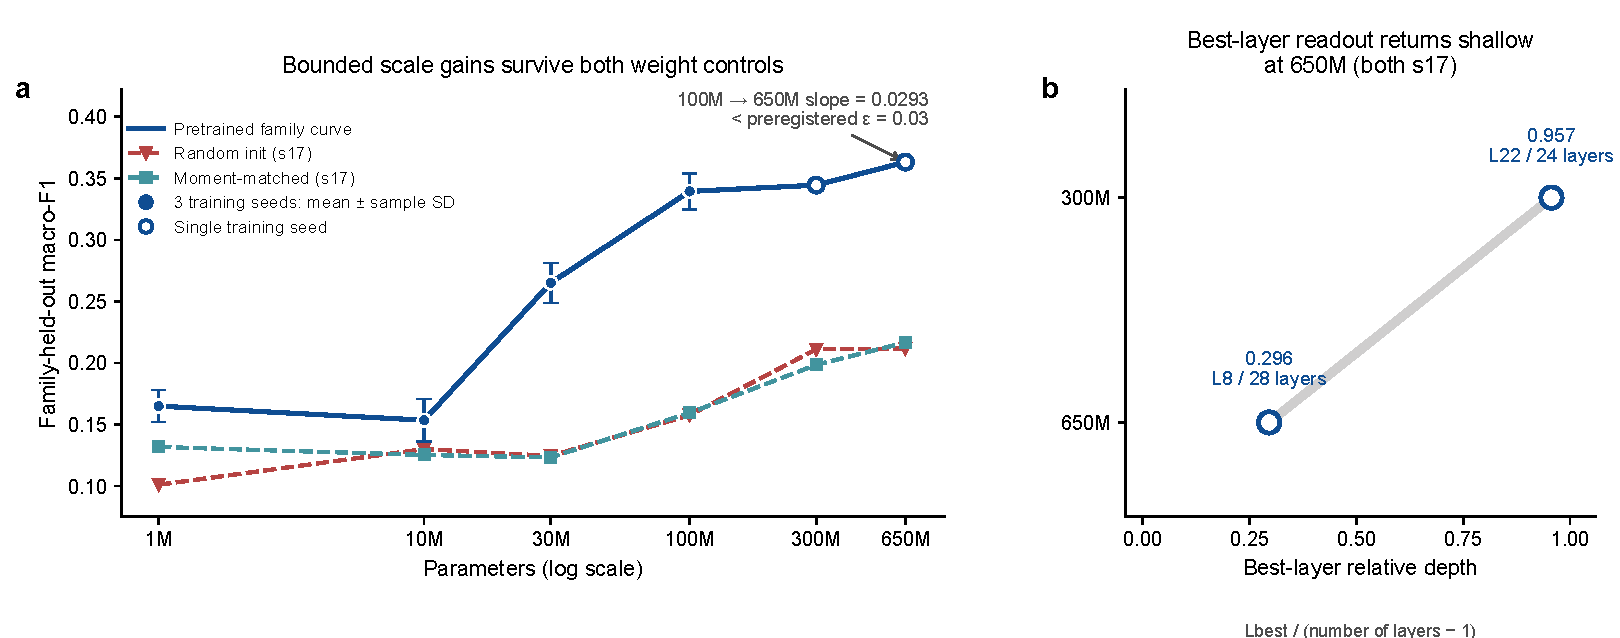
\includegraphics[width=\linewidth]{figs/fig1_q1q2_transfer_controls.pdf}
\caption{What does scale buy? Bounded, non-monotone family transfer. Is the gain real? Learned weights outperform architectural and weight-statistic controls.}
\label{fig:1}
\end{figure}

\hypertarget{what-is-the-learned-signal-worth-under-family-held-out-generalization-a-protocol-dependent-margin-above-composition}{%
\subsection{What is the learned signal worth under family-held-out generalization? A protocol-dependent margin above composition}\label{what-is-the-learned-signal-worth-under-family-held-out-generalization-a-protocol-dependent-margin-above-composition}}

This section asks how much the learned-weight advantage established in Section 4.2 is worth when evaluation requires generalization to held-out families. The decisive experiments are S9, crossing family and random splits with balanced and mean-pool readouts; a classical baseline group spanning k-mer logistic regression, k-mer LightGBM, a one-hot CNN, and a random-embedding head; and the S4-by-S9 attribution triangle across initialization controls, composition features, and splits. The random-split dividend under balanced probing rises from +0.055 to a post-30M plateau of +0.416 to +0.438, whereas the family-held-out margin over composition baselines is small at low scale and depends on the readout protocol.

The two-world results separate family overlap from scale itself. Under balanced probing, \(\Delta_{\mathrm{split}}=F1_{\mathrm{random}}-F1_{\mathrm{family}}\) reaches +0.4378 at 30M and remains between +0.4155 and +0.4364 thereafter. Mean-pool probing gives a different curve: its gap is near zero only at 1M and 10M (\(-\)0.0372 and +0.0006), then becomes positive from 30M onward (+0.1865 to +0.3950). Thus, the large balanced-probe dividend is not a universal property of every readout, and the older summary that mean pooling removes the gap does not describe the four larger scales. All entries in this split comparison are s17 observations within the same model and protocol; the random partition permits family overlap by construction, although neither probe partition was used for MLM pretraining.

\begin{longtable}[]{@{}
  >{\raggedright\arraybackslash}p{(\columnwidth - 8\tabcolsep) * \real{0.16}}
  >{\raggedleft\arraybackslash}p{(\columnwidth - 8\tabcolsep) * \real{0.21}}
  >{\raggedleft\arraybackslash}p{(\columnwidth - 8\tabcolsep) * \real{0.21}}
  >{\raggedleft\arraybackslash}p{(\columnwidth - 8\tabcolsep) * \real{0.21}}
  >{\raggedleft\arraybackslash}p{(\columnwidth - 8\tabcolsep) * \real{0.21}}@{}}
\toprule
Parameters & Balanced family F1 & Balanced random F1 & Balanced \(\Delta_{\mathrm{split}}\) & Mean-pool \(\Delta_{\mathrm{split}}\) \\
\midrule
\endhead
1M & 0.0982 & 0.1534 & +0.0552 & \(-\)0.0372 \\
10M & 0.1555 & 0.4928 & +0.3373 & +0.0006 \\
30M & 0.1675 & 0.6053 & +0.4378 & +0.1865 \\
100M & 0.1696 & 0.6040 & +0.4344 & +0.2283 \\
300M & 0.1715 & 0.5870 & +0.4155 & +0.3805 \\
650M & 0.1888 & 0.6252 & +0.4364 & +0.3950 \\
\bottomrule
\end{longtable}

Classical models show that much of this dividend is available without pretraining. K-mer logistic regression alone obtains \(\Delta_{\mathrm{split}}=+0.3549\), while the directly supervised one-hot CNN averages +0.3754 across three seeds. In contrast, the random-embedding head has almost no split dividend (+0.0036). These comparisons identify sequence composition and family overlap as sufficient ingredients for a large random-split gain, rather than treating a high random-split score as evidence of family-held-out generalization.

\begin{longtable}[]{@{}
  >{\raggedright\arraybackslash}p{(\columnwidth - 8\tabcolsep) * \real{0.17}}
  >{\raggedleft\arraybackslash}p{(\columnwidth - 8\tabcolsep) * \real{0.22}}
  >{\raggedleft\arraybackslash}p{(\columnwidth - 8\tabcolsep) * \real{0.22}}
  >{\raggedleft\arraybackslash}p{(\columnwidth - 8\tabcolsep) * \real{0.22}}
  >{\raggedright\arraybackslash}p{(\columnwidth - 8\tabcolsep) * \real{0.17}}@{}}
\toprule
Baseline & Family F1 & Random F1 & \(\Delta_{\mathrm{split}}\) & Seed coverage \\
\midrule
\endhead
k-mer (1--6) + logistic & 0.1630 & 0.5180 & +0.3549 & one fixed run, random\_state=17 \\
k-mer (1--6) + LightGBM & 0.1760 & 0.5485 & +0.3725 & s17 only \\
one-hot CNN & 0.1589 \(\pm\) 0.0119 & 0.5343 \(\pm\) 0.0253 & +0.3754 & three-seed mean \(\pm\) sample SD \\
random-embedding head & 0.0551 \(\pm\) 0.0253 & 0.0587 \(\pm\) 0.0103 & +0.0036 & three-seed mean \(\pm\) sample SD \\
\bottomrule
\end{longtable}

The family-world comparison nevertheless changes substantially with readout. Under the P0.3 primary caliber, mean-pool LM minus the strongest observed classical baseline, LightGBM s17 at 0.1760, is negative at 1M and 10M but positive from 30M onward. LightGBM has no s29 or s43 result, so these are not complete three-seed-versus-three-seed contrasts. At the four three-seed LM scales, the separate strict seed-coverage comparison instead uses the three-seed one-hot CNN mean; it yields +0.0061, \(-\)0.0054, +0.1062, and +0.1804. Seed coverage is matched in this column, but the different model types are not claimed to be paired experiments.

\begin{longtable}[]{@{}
  >{\raggedright\arraybackslash}p{(\columnwidth - 6\tabcolsep) * \real{0.20}}
  >{\raggedleft\arraybackslash}p{(\columnwidth - 6\tabcolsep) * \real{0.27}}
  >{\raggedleft\arraybackslash}p{(\columnwidth - 6\tabcolsep) * \real{0.27}}
  >{\raggedleft\arraybackslash}p{(\columnwidth - 6\tabcolsep) * \real{0.27}}@{}}
\toprule
Parameters & Mean-pool LM family F1 & LM \(-\) LightGBM s17, \(\Delta_{\mathrm{obs}}\) & Strict seed-coverage contrast, \(\Delta_{\mathrm{strict}}\) \\
\midrule
\endhead
1M & 0.1650 \(\pm\) 0.0131 & \(-\)0.0110 & +0.0061 vs CNN \\
10M & 0.1535 \(\pm\) 0.0173 & \(-\)0.0225 & \(-\)0.0054 vs CNN \\
30M & 0.2651 \(\pm\) 0.0162 & +0.0891 & +0.1062 vs CNN \\
100M & 0.3394 \(\pm\) 0.0147 & +0.1634 & +0.1804 vs CNN \\
300M & 0.3445 (s17) & +0.1685 & +0.1685 vs LightGBM s17 \\
650M & 0.3632 (s17) & +0.1872 & +0.1872 vs LightGBM s17 \\
\bottomrule
\end{longtable}

The balanced sensitivity analysis prevents this positive mean-pool slope from becoming an unconditional claim. At 100M, balanced-probe s17 scores 0.1696, exceeding k-mer logistic by only +0.0066 but falling below LightGBM s17 by \(-\)0.0064; mean-pool s17 instead scores 0.3263, or +0.1503 over the same LightGBM result. Consequently, the defensible family-held-out conclusion is protocol-specific: near-zero or negative margins occur at the two smallest mean-pool scales and in the 100M balanced comparison against LightGBM, while the primary mean-pool contrast turns positive at 30M and above. The 300M and 650M margins remain single-seed observations.

The attribution triangle then identifies what the balanced random dividend is made of. At 10M, random initialization captures 0.0380/0.3373 = 11.3\% of the trained dividend and moment-matched reinitialization captures 0.0412/0.3373 = 12.2\%; at 100M, random initialization captures 0.0795/0.4344 = 18.3\%. K-mer logistic captures 105.2\% of the 10M trained dividend and 81.7\% at 100M. Learned weights therefore matter for reading the family-overlap signal---untrained or moment-matched weights recover little of it---but composition features are sufficient for a classical model to reproduce most of that signal. Within these controlled cells, the random-split scale dividend is mainly a protocol-enabled, composition-level family-overlap phenomenon, not a measure of transferable knowledge acquired through scale.

\textbf{Strongest alternative explanation (B3).} The initialization controls and composition baselines do not establish that the remaining family-world LM signal is distinct from composition reading: both may exploit the same underlying sequence statistics. The controlled triangle supports attribution of the random-split dividend, but it cannot decompose the learned family-world representation into composition and non-composition components.

\begin{figure}[htbp]
\centering
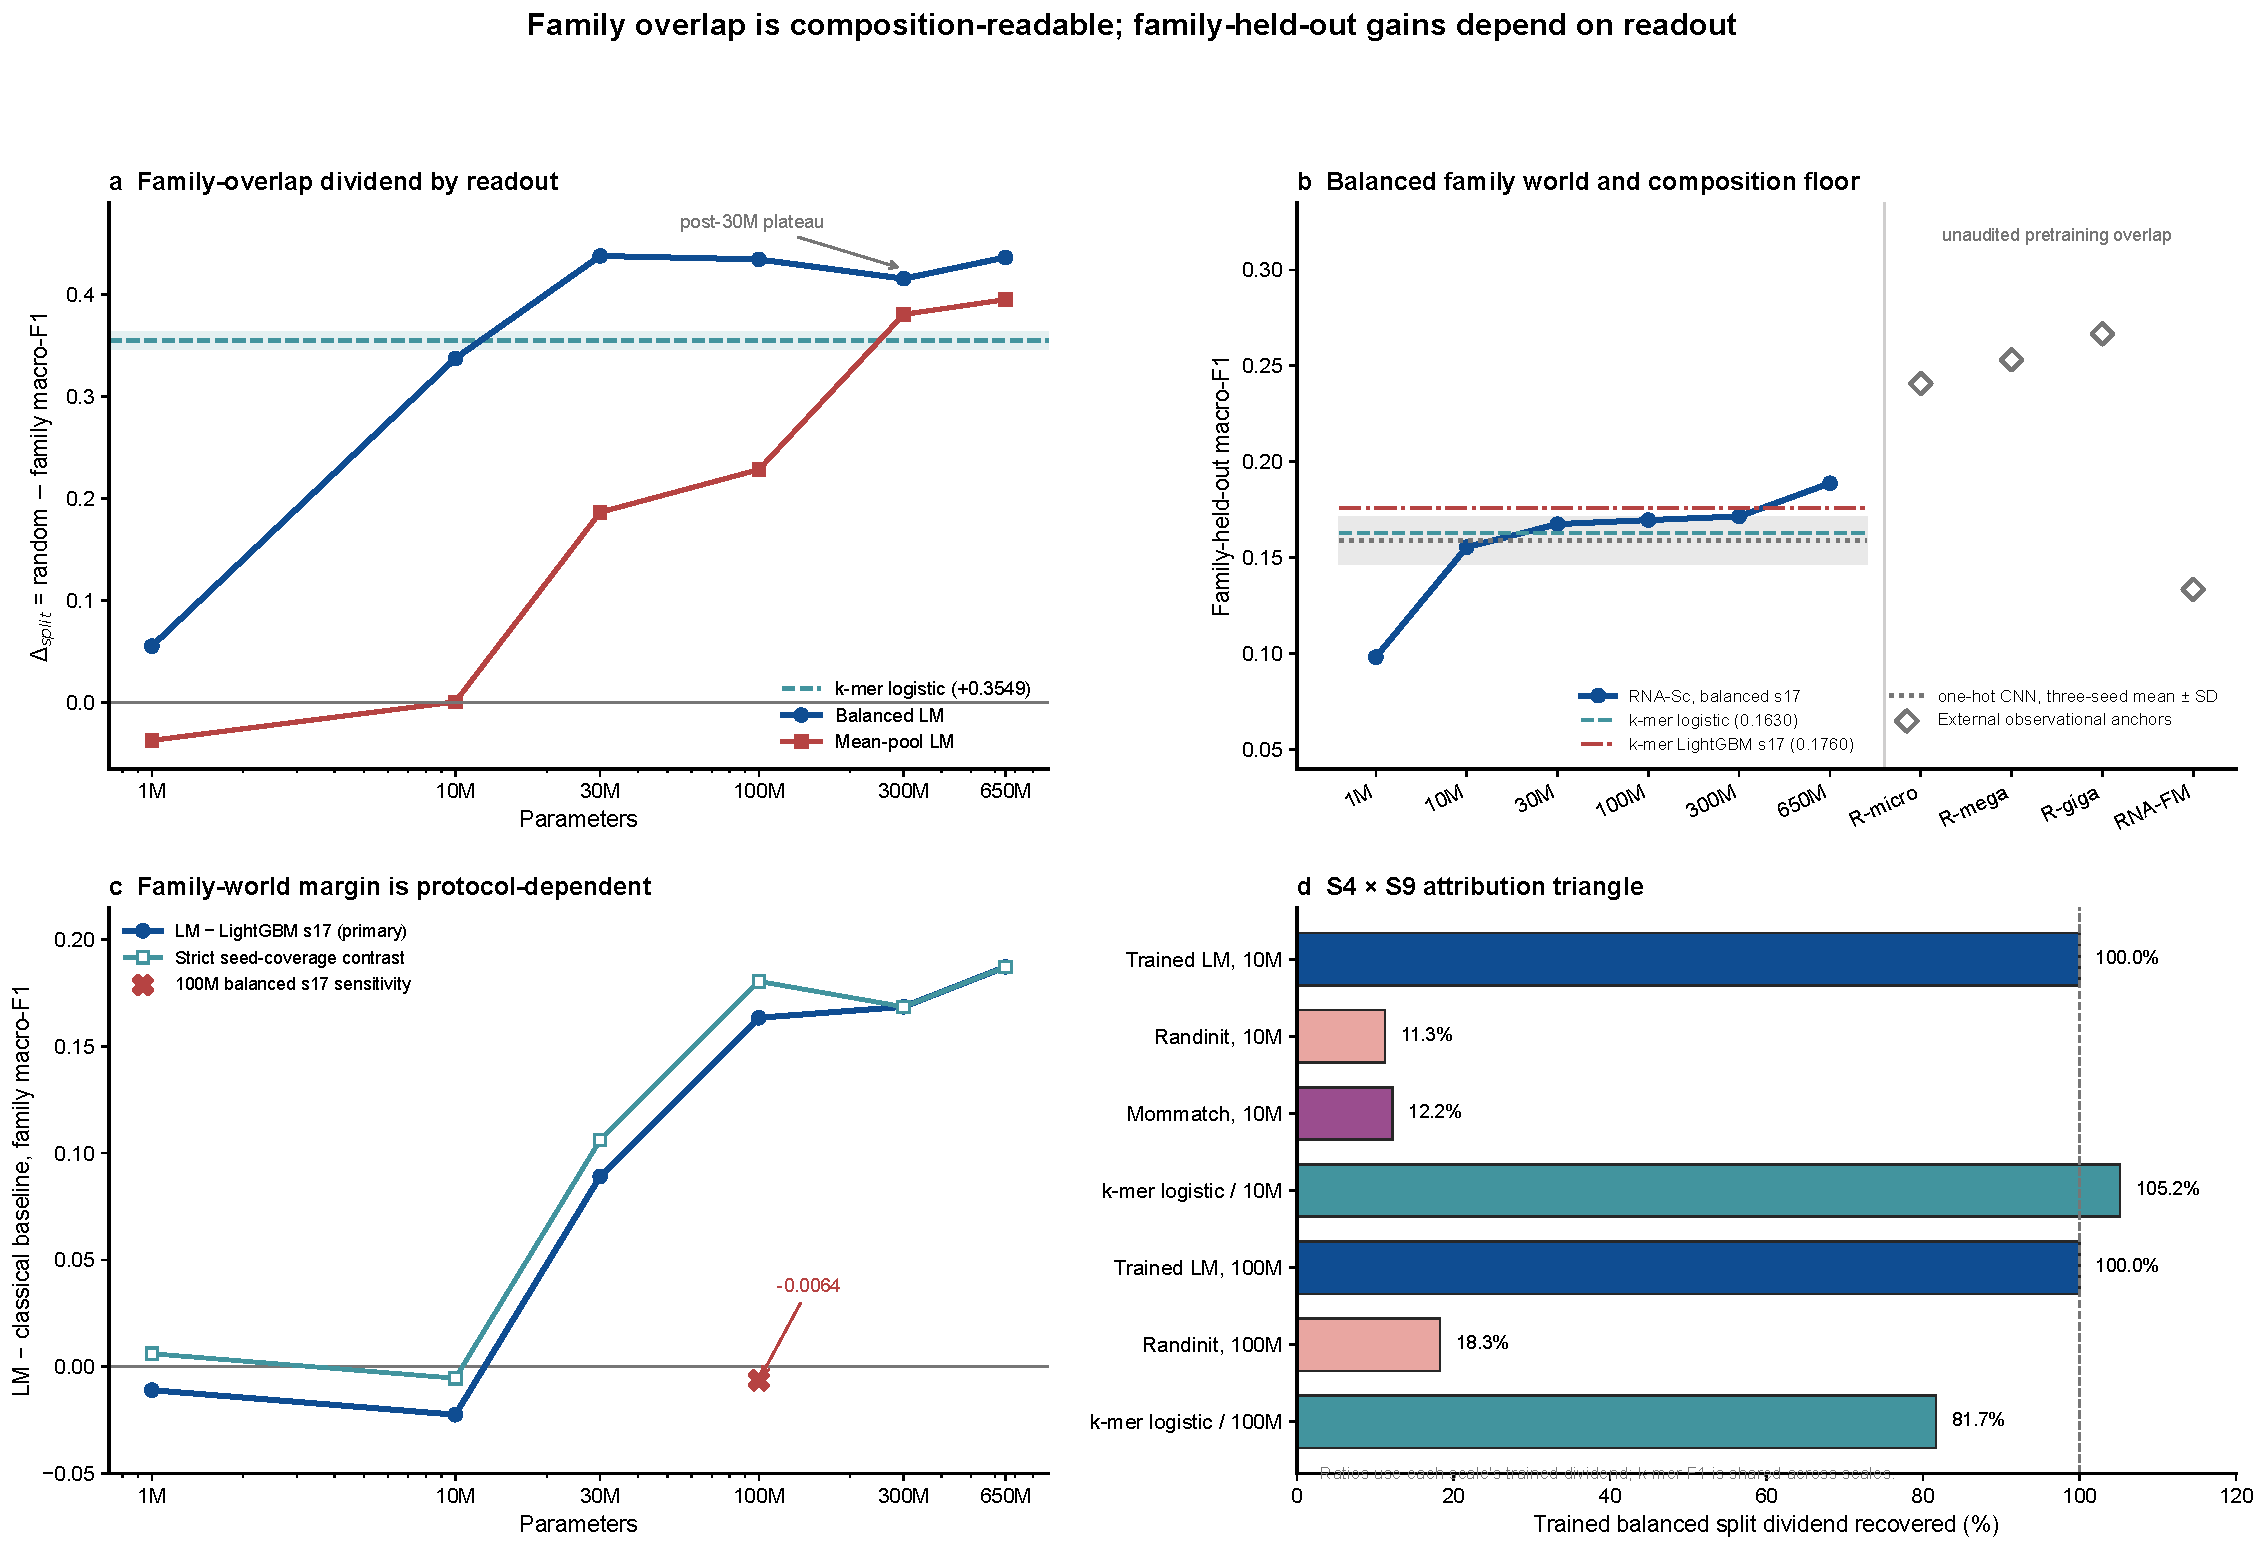
\includegraphics[width=\linewidth]{figs/fig2_q3_dualworld.pdf}
\caption{What is pretrained transfer worth under family-held-out generalization? (a) Random-minus-family macro-F1 under balanced and mean-pool readouts, with the k-mer logistic dividend as a reference band. (b) Balanced family-world scores for the controlled s17 ladder and classical baselines; external RiNALMo micro/mega/giga (0.2407/0.2532/0.2667) and RNA-FM (0.1335) points are observational anchors only because their pretraining exposure to the evaluation families cannot be audited. (c) Mean-pool LM margins over LightGBM s17, strict seed-coverage contrasts, and the 100M balanced sensitivity point; the LightGBM baseline is single-seed and no uncertainty is imputed. (d) Percentage of the trained balanced random-split dividend recovered by initialization controls and k-mer logistic. Together, the panels distinguish a composition-reproducible protocol dividend from the smaller, readout-dependent family-world margin.}
\label{fig:2}
\end{figure}

The location of this protocol-dependent transferable signal now forces the next question: where in the network does it reside, and why does readable family signal erode at 10M and return to shallower layers at 650M? This section cannot localize that signal, explain its training dynamics, separate learned family-world structure from composition reading (B3), or establish training-seed robustness at 300M and 650M.

\hypertarget{where-does-the-signal-reside-and-why-does-it-erode-or-return-to-shallow-layers}{%
\subsection{Where does the signal reside, and why does it erode or return to shallow layers?}\label{where-does-the-signal-reside-and-why-does-it-erode-or-return-to-shallow-layers}}

This section asks where transferable family signal becomes readable and why prolonged training produces attrition at 10M but a shallow readout optimum at 650M. The decisive experiments are the S6 checkpoint trajectories and S7 layer-wise probes, S12 stratification by the family decoupling index (DI), the pre-registered P1 rRNA-class-removal intervention, and P5 native-versus-shuffled likelihood separation, with P4 testing quantitative extrapolation. Family signal rises and then erodes during 10M training while its best layer moves downward, whereas removing rRNA from the 650M probe task restores a deepest-layer optimum.

The family-level signal isolated by the preceding split-and-baseline analysis is therefore not a static, uniformly deep representation. The frozen S6 analysis covers 37 checkpoints; in the full-corpus 10M s17 trajectory, macro-F1 reaches 0.2549 at 0.5B nt and then falls to an approximately 0.173 plateau, ending at 0.1731 at 1.9B nt. The best layer is L16 at the first 0.1B checkpoint, L11 at the 0.5B maximum, and L1 at the terminal checkpoint, showing that score attrition and readout relocation accompany one another.

The c1Mcs arm separates exposure duration from epoch count within this comparison. At 2.22 epochs, it reproduces the rise and decline: macro-F1 peaks at 0.2437 at 0.5B nt, falls to 0.2042 at 0.7B, and ends at 0.1862 at 0.9B; the best layer moves from L16 at 0.3B to L6 at 0.7B, finishing at L9. Thus, repetition count alone does not explain the erosion: a similar exposure-time pattern occurs in arms with approximately 0.14 and 2.22 epochs. This supports duration-dependent attrition within the evaluated arms, although differences in unique-corpus composition remain an alternative contributor. Moreover, the trajectory is a single s17 run; it does not make the terminal 10M mean-level dip universal across training seeds.

S7 shows that this attrition is task-specific rather than a general collapse of every readable feature. The paired-position secondary-structure probe does not exhibit the corresponding 10M scale collapse seen for family classification. This negative result narrows the phenomenon to the family-readout channel, but neither the absolute structure score nor its layer-wise linear readout can determine how much pairing knowledge the encoder contains.

S12 then asks which families occupy which depths. Across the 10 class-level aggregates, Spearman's correlation between DI and best-layer relative depth is \(-\)0.478 for 30M-c1Mcs, \(-\)0.384 at 100M, \(-\)0.339 at 300M, and \(-\)0.222 at 650M. The negative sign means that high-DI, structure-conserved but sequence-divergent families tend to peak earlier; the association attenuates monotonically toward zero with scale. These are descriptive E1 correlations over only 10 classes, not family-level inferential estimates, and the 30M point belongs specifically to the c1Mcs arm.

We organize these observations with \textbf{hypothesis M, a post-hoc grade-B account} comprising three proposed links: (a) diminishing marginal non-rRNA benefit from depth, (b) increasing dominance of the corpus-majority rRNA channel in deep-layer readout as capacity grows, and (c) a depth-dependent random-mixing floor that reduces deep-layer signal-to-noise. Links (a) and (c) remain descriptive; only link (b) is targeted by a controlled intervention. The hypothesis is therefore an interpretation to be constrained, not an established capacity-reallocation mechanism.

The pre-registered P1 intervention removes the rRNA class from probe training and evaluation, yielding an 18-class task while leaving the pretrained encoders unchanged. At 100M, the full-class and de-rRNA optima are L21 (relative depth 0.955) and L16 (0.727), respectively; at 300M they are L22 (0.957) and L18 (0.783). Most importantly, the 650M optimum moves from L8 (0.296) in the full-class task to L27 (1.000) after rRNA removal, completely abolishing the shallow-endpoint reversal. De-rRNA macro-F1 also increases monotonically across these scales---0.3192, 0.4026, and 0.4585---with the 650M value the highest in this 18-class arm. These F1 values are not directly comparable with the 19-class full-task scores. Within this probe-class intervention, P1 provides E2 evidence that rRNA inclusion causally contributes to the shallow 650M optimum and that deep layers retain readable non-rRNA family features, supporting chain (b) without validating chains (a) or (c).

P5 supplies a zero-supervision boundary on that interpretation. Native-minus-shuffled MLM separation at 30M and 650M is 1.0668 and 1.1184 nats/token for rRNA, but rises from 0.1267 to 0.3098 for non-rRNA; the corresponding rRNA-minus-non-rRNA gap \textbf{narrows} from 0.9401 to 0.8086. P5b's predicted widening gap is therefore refuted, ruling out increasingly dominant rRNA likelihood separation as the explanation for the 650M reversal. The 30M random-initialization control has separations of only 0.0018 and 0.0004, respectively, so the measured separations require learned sequence structure; nevertheless, P5 does not undo the distinct P1 class-removal result.

P4 further rejects a simple quantitative completion of hypothesis M. Leave-one-out extrapolation from de-rRNA to full-class best-layer position has mean error 0.3046 for a linear map and 0.7447 for a capacity-shift map, with the latter exceeding 1.0 at both 10M and 650M. The resulting verdict is deliberately limited: chain (b) has intervention support, chains (a) and (c) remain descriptive, P5b refutes the widening-gap prediction, and the tested quantitative forms fail; no general capacity-to-layer law is established.

\begin{figure}[htbp]
\centering
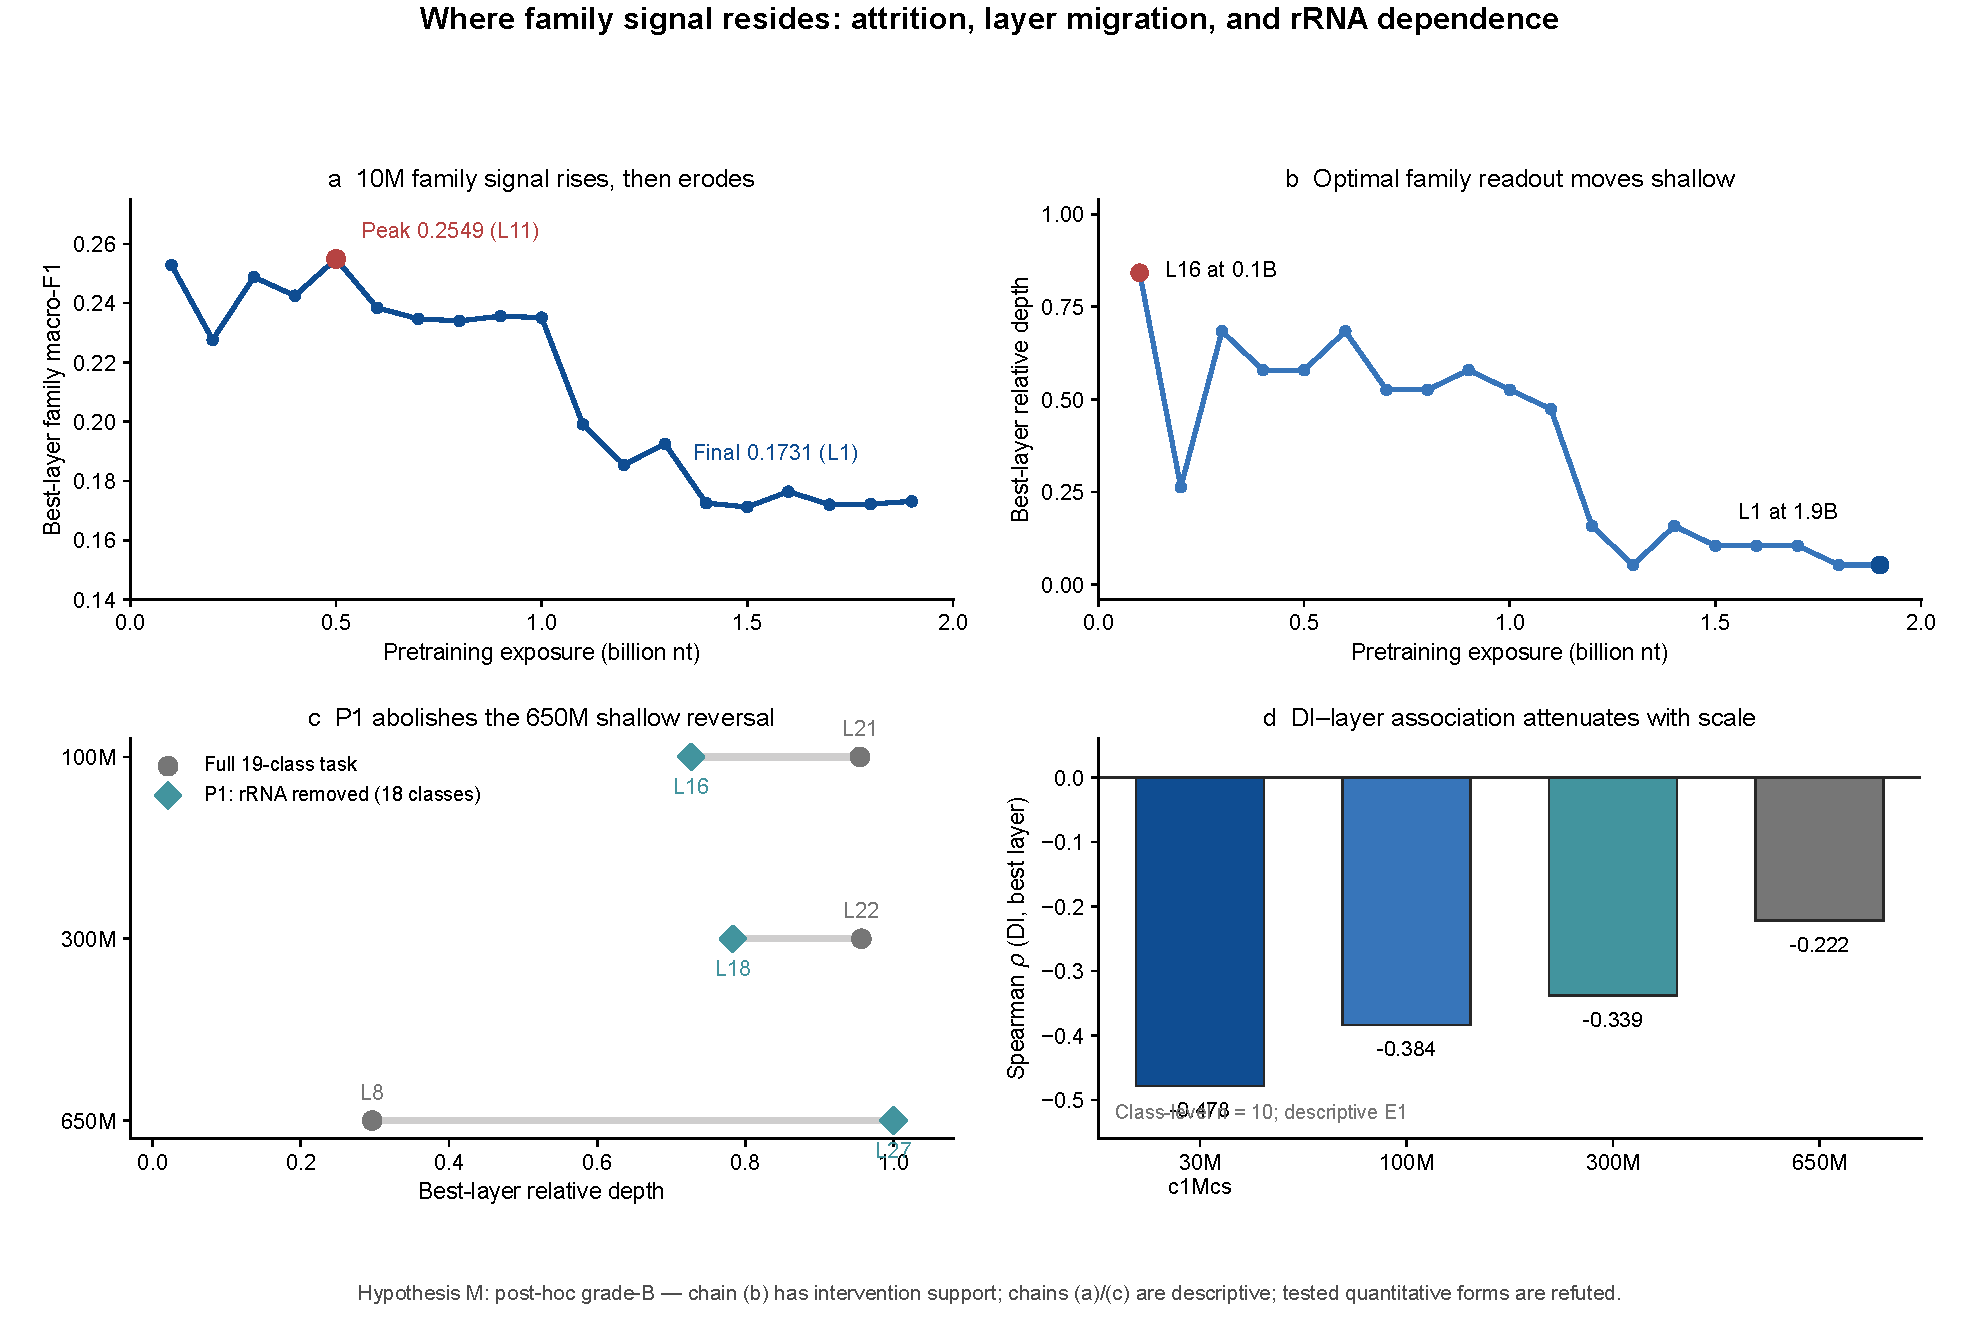
\includegraphics[width=\linewidth]{figs/fig3_q4.pdf}
\caption{Attrition, layer migration, P1 intervention, and DI stratification. Figure 3 answers where family signal becomes readable and how rRNA changes its optimal depth. (a) The 10M s17 family macro-F1 trajectory rises to 0.2549 at 0.5B nt before eroding to 0.1731 at 1.9B nt. (b) Its best-layer relative depth moves from 0.842 (L16) at 0.1B to 0.053 (L1) at the terminal checkpoint. (c) P1 rRNA-class removal changes the full-class versus 18-class de-rRNA optima at 100M, 300M, and 650M; class-removal F1 values are not compared across class sets. (d) The DI--best-layer Spearman correlation attenuates from \(-\)0.478 to \(-\)0.222 across the four evaluated arms (class-level \(n=10\), E1). Points denote single s17 runs without training-seed intervals. Hypothesis M is post-hoc grade-B: chain (b) receives intervention support, chains (a) and (c) remain descriptive, and its tested quantitative forms are refuted.}
\label{fig:3}
\end{figure}

This layer- and channel-dependent family readout forces the next question: does weak secondary-structure linear probing reflect knowledge that was never acquired, or pairing knowledge that this readout cannot recover? This section cannot answer that question, establish hypothesis M as a complete mechanism, or generalize the single-run attrition trajectory across training seeds.

\hypertarget{is-structural-knowledge-absent-or-inaccessible-pairing-is-learned-but-partner-finding-is-the-bottleneck}{%
\subsection{Is structural knowledge absent or inaccessible? Pairing is learned, but partner finding is the bottleneck}\label{is-structural-knowledge-absent-or-inaccessible-pairing-is-learned-but-partner-finding-is-the-bottleneck}}

The layer relocation in Section 4.4 leaves open whether the small structural-probe increments reflect missing pairing knowledge or a readout failure. The decisive experiments form a five-stage chain: GC and trigram composition floors, probe-free covariation mutations, same-layer readout replacement, a Partner-Oracle, and candidate-pair probes evaluated against a matched composition-and-distance prior. Together they show small but genuine pretraining-derived pairing signal whose measured magnitude depends sharply on the readout channel.

\textbf{Composition floors calibrate the linear-probe result.} The S7 task predicts paired positions, so its macro-F1 must first be compared with sequence-composition rules rather than interpreted as a direct measure of structural knowledge. A GC-identity rule attains 0.576/0.608/0.599 on bpRNA-TS0, bpRNA-val, and ArchiveII, respectively, while the stronger left--center--right trigram baseline attains 0.592/0.616/0.621. A probe trained once on bpRNA-TR0 and evaluated unchanged on all three sets leaves the following increments above the corresponding trigram floors:

\begin{longtable}[]{@{}lrrr@{}}
\toprule
Scale & TS0 \(-\) trigram & val \(-\) trigram & ArchiveII \(-\) trigram \\
\midrule
\endhead
1M & +0.001 & \(-\)0.006 & +0.004 \\
10M & +0.013 & +0.001 & +0.019 \\
30M & +0.024 & +0.021 & +0.033 \\
100M & +0.017 & +0.011 & +0.032 \\
650M & +0.034 & +0.046 & +0.038 \\
\bottomrule
\end{longtable}

The increment is therefore small but reappears across all three evaluation sets at 650M. It is also distinct from a same-layer trained-minus-random comparison: when each arm selects its own best layer in the single-set full scans, trained-minus-randinit is +0.007/\(-\)0.001/\(-\)0.003/+0.004 at 1M/10M/30M/100M. Thus, through 100M, pretraining mainly changes where pairing-related signal is linearly readable rather than raising the best-layer linear ceiling. The much larger same-layer contrast at 650M is not used as a knowledge estimate because the untrained deep representation itself collapses, conflating signal content with layer readability. These single-run probe comparisons calibrate the composition floor; they do not provide training-seed replication for a structural scaling law.

\textbf{Forward covariation separates knowledge from linear readability.} The mutation test masks position \(j\), changes its true partner \(i\) to an alternative nucleotide, and measures the probability shift at \(j\) toward the new complement (COV). An unpaired-position control (CTRL) tests the corresponding composition response, with 4,920 mutation events per arm. Random initialization preserves the architecture but removes pretraining.

\begin{longtable}[]{@{}lr@{}}
\toprule
Arm & COV \(-\) CTRL \\
\midrule
\endhead
1M trained & +0.00415 \\
10M trained & +0.00504 \\
30M trained & +0.01121 \\
100M trained & +0.02030 \\
300M trained & +0.04694 \\
650M trained & +0.09572 \\
30M randinit & +0.00007 \\
650M randinit & +0.00004 \\
\bottomrule
\end{longtable}

The response increases throughout the controlled ladder and is 4.7-fold larger at 650M than at 100M. At 650M, the probability assigned to the old complement simultaneously falls by 0.10227, approximately balancing the shift toward the new complement. The unpaired control and the near-zero random-initialization responses exclude the tested composition shortcut and architectural prior within this assay. Pairing-dependent probability structure is therefore present in the forward pass and arises from pretraining, even when a per-position linear probe exposes only a small increment; the probe value is a lower bound on readable knowledge, not a measure of all forward-pass knowledge.

\textbf{External COV provides observational cross-model corroboration.} Under the same mutation protocol, COV \(-\) CTRL is +0.1134/+0.1998/+0.2477 for RiNALMo micro/mega/giga and +0.0108 for NucleicBERT; every corresponding randinit17 control is approximately zero. RNA-Sc-650M's +0.0957 lies between RiNALMo micro and mega, while the RiNALMo gradient rises with external model scale. These are observational anchors across confounded architectures, corpora, and exposures, not controlled scale attribution. The 300M sanity rerun passed protocol-equivalence checks; its small cross-hardware/software residual is reported with a \texttt{1e-4} hardware-tolerance note, without claiming a uniquely proven cause because the exact old environment was not retained.

\textbf{Replacing the readout locates the wall at partner finding.} Holding the layer, training data, evaluation set, metric, and class weighting fixed, we replace the linear head with local symmetric pooling (pool16), attention, or symmetry-constrained attention (attn\_symm). A separate arm unfreezes the final two encoder layers, while Partner-Oracle supplies the true partner state and thus serves only as an information-access upper bound.

\begin{longtable}[]{@{}lrrrrrr@{}}
\toprule
Scale (layer) & Linear & pool16 & attn & attn\_symm & Fine-tune top 2 & Partner-Oracle \\
\midrule
\endhead
30M (L3) & 0.6120 & 0.6413 & 0.6295 & 0.6285 & 0.6260 & 0.9996 \\
100M (L22) & 0.6212 & 0.6218 & 0.6214 & 0.6354 & 0.6368 & 0.9992 \\
650M (L15) & 0.6101 & 0.6151 & 0.6291 & 0.6348 & 0.6405 & 0.9983 \\
\bottomrule
\end{longtable}

Remote interaction improves readout, with pool16 preferred at the shallow 30M layer and symmetrized attention preferred at the two deeper layers. Yet every method that must identify the partner remains near 0.64, including end-to-end adaptation of the top two layers, whereas supplying the true partner raises macro-F1 to at least 0.998 at every tested scale. This controlled contrast localizes the immediate bottleneck: the two endpoints jointly contain information sufficient for the Oracle readout, but generic per-position heads and limited fine-tuning do not recover the partner search. The Oracle is not a deployable predictor, and its ceiling does not imply that an automatically generated partner set will retain the same accuracy.

\textbf{Candidate-pair scoring confirms the diagnosis after prior correction.} The pair-level probe changes the task from isolated position classification to scoring \((h_i,h_j,|i-j|)\) as paired or unpaired. Raw candidate-ranking AUC is high, but a model-free baseline using distance, endpoint positions, nucleotide identities, and complement status already reaches 0.922; the meaningful model contribution is the increment above this matched prior.

\begin{longtable}[]{@{}lrrr@{}}
\toprule
Scale & Pair AUC & AUC \(-\) matched prior & Pair-probe top-L precision \\
\midrule
\endhead
30M & 0.9319 & +0.0099 & 0.0319 \\
100M & 0.9397 & +0.0177 & 0.0563 \\
650M & 0.9524 & +0.0304 & 0.0641 \\
\bottomrule
\end{longtable}

Candidate conditioning therefore reveals a real, scale-increasing increment that the per-position wall conceals, with the largest net gain at 650M. Within these assays, the immediate missing component is a pairing solver for candidate generation and matching, not simply additional pretraining; this diagnoses the present bottleneck without predicting how accurate such a solver would be. It does not solve structure prediction: top-L precision remains low, and the 650M dynamic-programming pair-F1 of 0.2000 does not exceed its randinit value of 0.2104, confirming that the downstream pairing solution remains prior-dominated. Pair AUC, pair-probe top-L precision, dynamic-programming pair-F1, and paired-position macro-F1 are kept as distinct metrics rather than treated as interchangeable structure scores.

An independent long-range contact probe gives the same qualified conclusion under yet another metric. For pairs separated by at least 24 nt, APC-corrected top-L precision reaches 1.19/1.28/1.53 times chance at 30M/100M/650M, compared with 1.06/0.92/1.31 for randinit; thus the 650M trained-minus-randinit excess is 0.22-fold chance. The absolute values remain close to chance under this sequence-level bpRNA split, so the result supports weak pretraining-derived pairing geometry, not accurate long-range contact prediction.

\textbf{Probe-free batteries corroborate coupling but retain their boundary results.} On 80 bpRNA-TS0 sequences of length at most 128 nt, masked-logit interaction (MLI) at RNA-Sc-650M averages +0.158 for paired positions versus \(-\)0.001 for distance-matched controls, giving pair-versus-control AUC 0.743; randinit yields AUC 0.492. This independently supports learned pairwise coupling without training a structural probe. Attention provides descriptive rather than causal localization: the strongest pair-tracking ratio occurs early in the ALiBi model (L6-H0, 16,140-fold), whereas a learned-positional-encoding external anchor shows its reported maximum in a deep head (L27-H8, 617-fold). This observational contrast warns against treating a universal layer location as the mechanism. Finally, boundary saliency is weak in RNA-Sc-650M (0.000174 at boundaries versus 0.000166 in interiors) and shows no zero-shot boundary elevation in the external anchor. That negative result bounds the interpretability claim: input-gradient magnitude need not register a distributed partner-matching computation, so weak saliency does not overturn the controlled covariation and MLI evidence, but neither does it provide independent support for boundary encoding. Figure 4 summarizes the full chain from composition floors to prior-corrected pair readout.

Having established that structural knowledge can be present yet hidden by partner finding, the next question is what controls its supply: does family-channel saturation also bound structure, or do corpus composition and budget affect the two channels differently? This section does not show that current representations suffice for accurate structure prediction, that adding a pairing solver will close the gap, or that the readout wall generalizes across architectures and external pretraining corpora.

\begin{figure}[htbp]
\centering
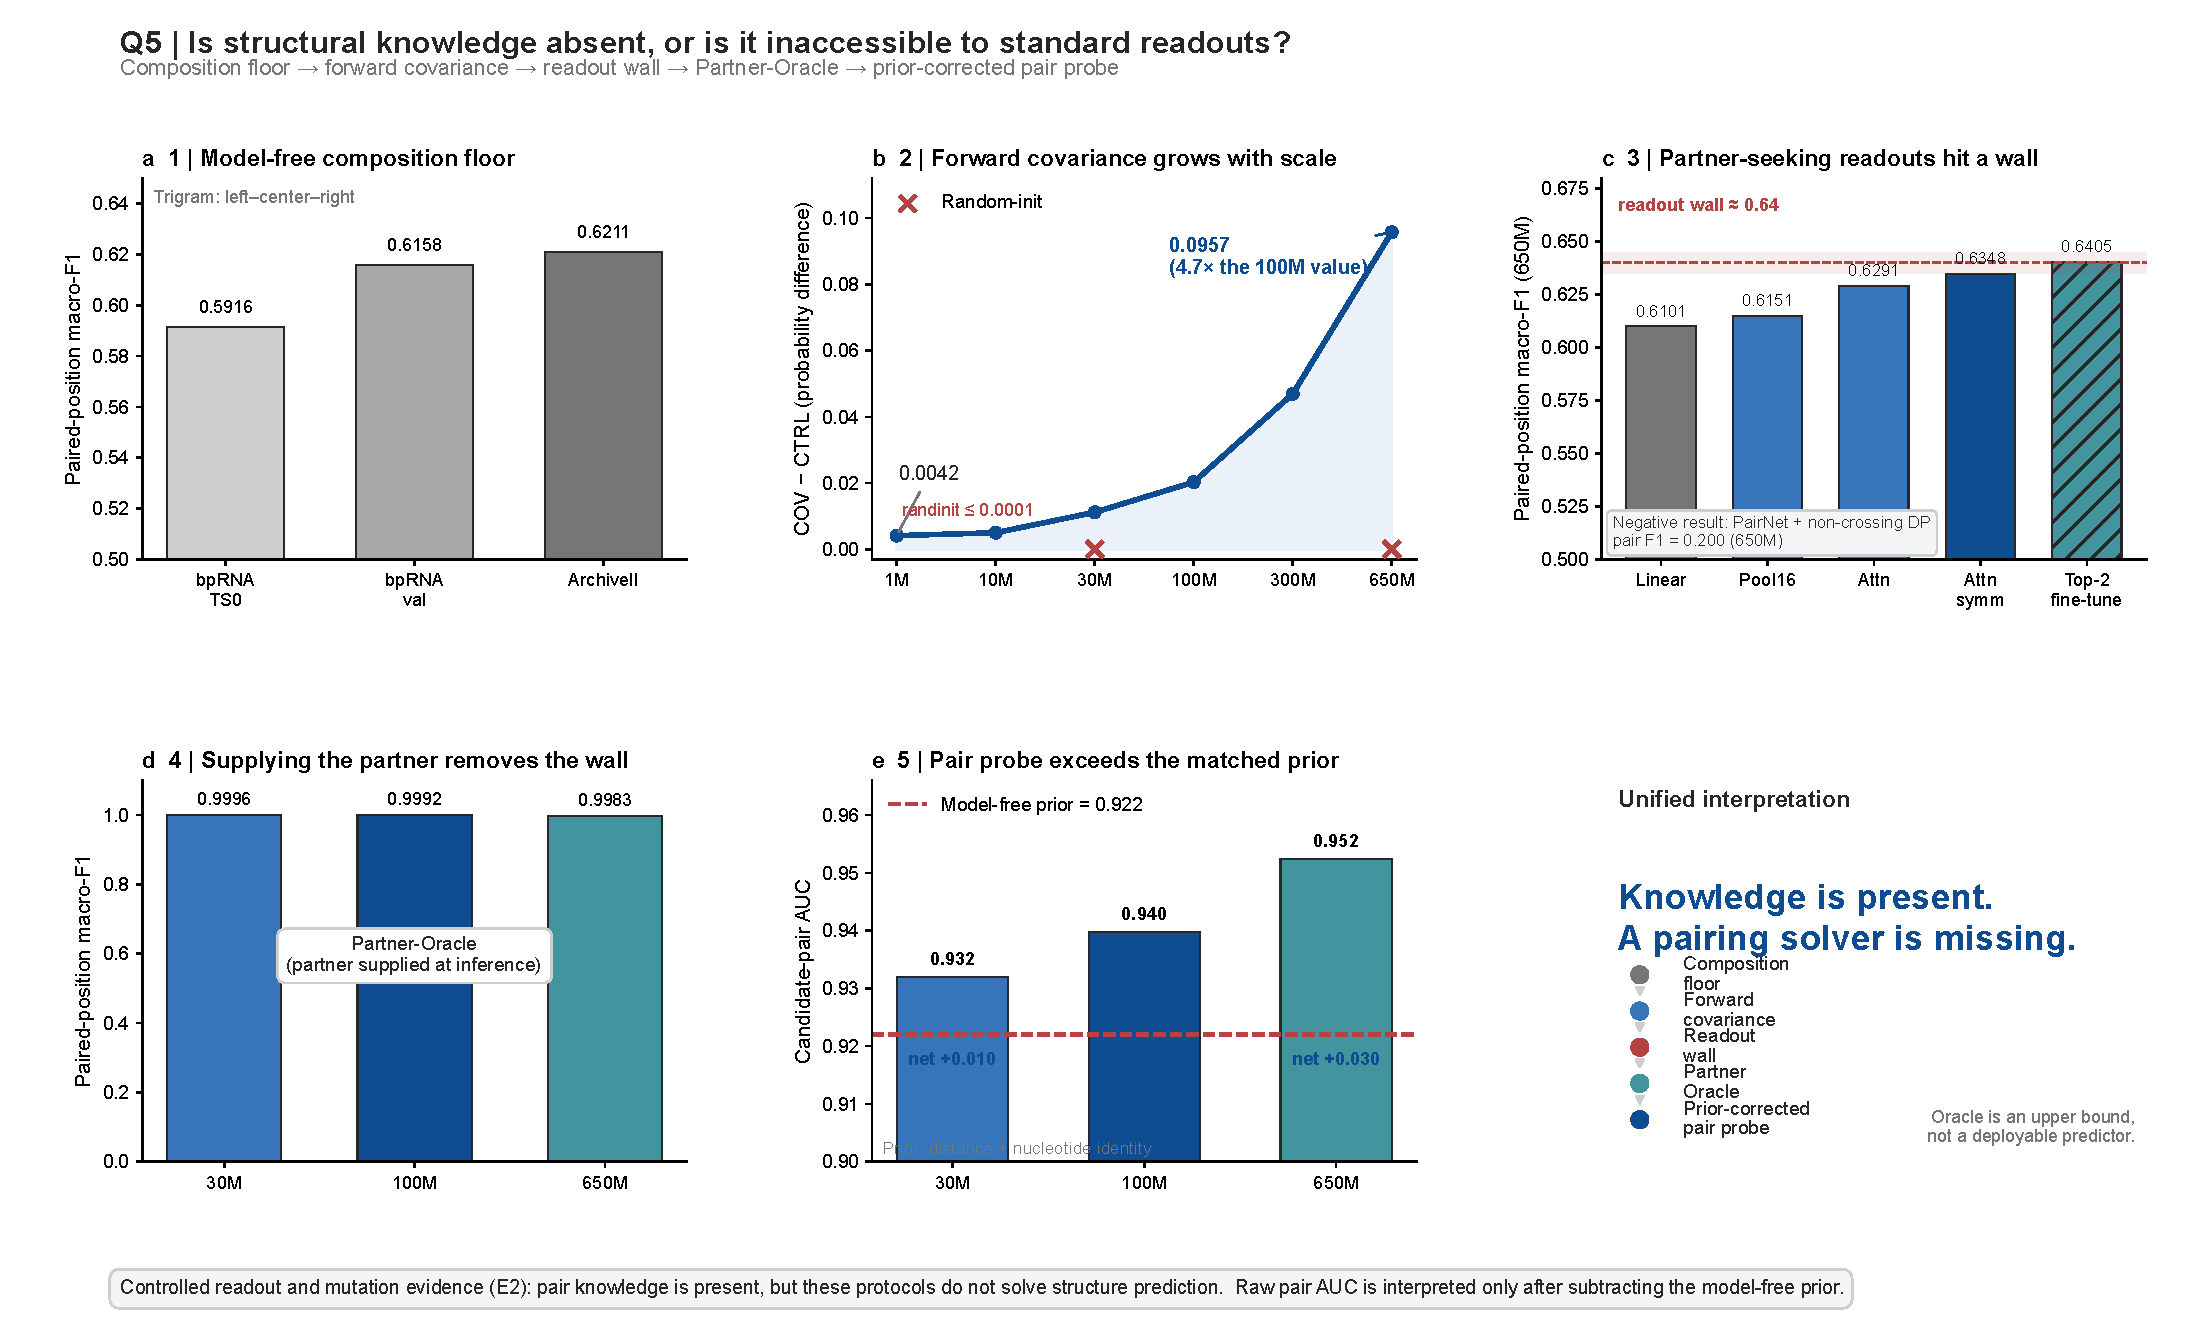
\includegraphics[width=\linewidth]{figs/fig4_q5_readout_chain.pdf}
\caption{Is structural knowledge absent or inaccessible? Pairing is learned, but partner finding is the bottleneck.}
\label{fig:4}
\end{figure}

\hypertarget{what-determines-knowledge-supply-corpus-composition-budget-position-and-scale}{%
\subsection{What determines knowledge supply? Corpus composition, budget position, and scale}\label{what-determines-knowledge-supply-corpus-composition-budget-position-and-scale}}

This section asks what determines the supply of transferable knowledge after \S4.5 showed that structural knowledge can be present yet gated by readout. The decisive experiments manipulate unique-corpus size (S2), family-frequency diversity (S3/rw1), corpus recipe at fixed architecture and budget, exposure budget across scale, and Rfam enrichment, with family, random-split, structure, RNS, and P5 channels as readouts. Supply is governed by a corpus-composition \(\times\) budget \(\times\) scale interaction: small models can be hurt by excess exposure, larger models can benefit, and corpus-replacement gains shrink as capacity grows.

\textbf{Unique-token count is not a sufficient measure of supply.} S2 varies unique-corpus size while holding total pretraining exposure fixed. At 30M, the c1M arm reaches family macro-F1 0.3160 with 0.85B unique nucleotides and 2.35 epochs, exceeding both the full-corpus three-training-seed mean of 0.2651 and the matched-s17 full-corpus value of 0.2466. The comparison of corpus arms is therefore between s17 runs, whereas the 0.2651 value supplies the broader seed-mean context; these coverage levels are not interchangeable. The validation-loss ranking is inverted relative to transfer F1, so a lower MLM validation loss does not identify the corpus with greater family-level supply. Within this axis, effective repetition of useful family statistics predicts transfer better than unique-token coverage alone.

\textbf{Composition interventions reveal a capacity gate.} The rw1 arm flattens the family-frequency sampling prior without changing the architecture, budget, or evaluation set, while the recipe-replica arm replaces the corpus under the same architecture and 2.0B-nt exposure. Rfamcap provides an orthogonal Rfam-enriched contrast. Their family-probe effects are summarized below in percentage points.

\begin{longtable}[]{@{}lrrrr@{}}
\toprule
Controlled corpus arm & 10M & 30M & 100M & 300M \\
\midrule
\endhead
Family-prior flattening (rw1) & +0.15 (neutral) & \(-\)0.58 & \(-\)4.29 & --- \\
RiNALMo-recipe replica & --- & +7.93 & +2.33 & +0.63 \\
Rfam enrichment (rfamcap, terminal iso-budget) & --- & +4.14 & +0.34 & --- \\
\bottomrule
\end{longtable}

Entries are arm-minus-control differences in best-layer family macro-F1 for matched s17 runs. The rw1 and recipe-replica contrasts are controlled interventions (E2); rfamcap remains a single-seed orthogonal arm (E1). The rw1 effect at 10M is smaller than the 10M training-seed SD of 0.0173 and is therefore neutral rather than evidence of a positive effect. Its sign reversal at larger scales rejects a universal benefit of diversity flattening within these interventions: once capacity is sufficient, flattening can remove family-frequency structure that the model would otherwise exploit. The recipe-replica gains decay monotonically from +7.93 to +0.63 pp, directly confirming a corpus-composition lever whose return depends on capacity. This is a recipe replica, not an exact reconstruction of the original sequence manifest. A secondary contact readout at 100M points in the same direction, with top-L precision over chance rising from 1.28\(\times\) to 1.40\(\times\) (+9\%); this near-chance contact metric is directional support and is not mixed with paired-position macro-F1.

\textbf{Budget interacts with scale rather than defining a single corpus ceiling.} The pre-registered factorial repeats the 30M, 100M, 300M, and 650M runs at 5.9B nt under the original terminal-checkpoint protocol. The three readout channels respond differently to the same intervention, but the random channel has terminal results only at the three smaller scales.

\begin{longtable}[]{@{}lrrr@{}}
\toprule
Scale & Family \(\Delta\)F1 (pp) & Structure \(\Delta\)F1 (pp) & Random-split \(\Delta\)F1 (pp) \\
\midrule
\endhead
30M & \(-\)5.24 & +0.09 & +0.65 \\
100M & \(-\)2.74 & +0.85 & \(-\)0.60 \\
300M & +3.76 & +1.87 & +4.10 \\
650M & +1.15 & +0.84 & --- (terminal not evaluated) \\
\bottomrule
\end{longtable}

For family transfer, the effect is negative at 30M and 100M but positive at 300M and 650M, with the positive return attenuating at 650M. Thus 2.0B nt is already beyond the useful budget for the smaller family-classification models but is insufficient at larger scales. Claim-14 predicted a 300M budget gain below 1.0 pp; the observed +3.76 pp falsifies that pre-registered boundary (E3), replacing a hard corpus-limit account with a scale-dependent budget position. The 650M +1.15 pp effect and the observation that added budget helps an undertrained larger scale are single-seed E1 results under the original terminal protocol, not training-seed-replicated estimates.

The structure channel increases monotonically over 30M--300M (+0.09/+0.85/+1.87 pp) and remains positive but falls back at 650M (+0.84 pp), so the monotone statement is restricted to three scales. Moreover, a budget difference is not itself a learning increment: after subtracting randinit, only the 100M and 300M models at 5.9B exceed the approximately 1 pp repeat-noise reference, with learning increments of +1.07 and +2.66 pp, respectively. The random-split channel shows no family-like erosion and no coherent dose-response at the three completed terminal comparisons (+0.65/\(-\)0.60/+4.10 pp). We use ``budget-insensitive'' only for this three-scale terminal pattern in sign and mechanism, not to claim that every magnitude lies within \(\pm\)2 pp or that the unevaluated 650M terminal response is known. The 650M 5B midpoint is retained solely as a historical appendix observation because P2.7 terminal consolidation is not performed.

Under the original full-layer 20k/4k protocol, 650M at 5.9B scores 0.3747 versus 0.3821 for 300M. The separate deep-window retest is not a current result: it is demoted to an unreviewed handover-record citation in Appendix A because its raw ledger is incomplete and cannot be adjudicated with an authoritative reconstructed split. No retest or cross-protocol difference is substituted for the +1.15 pp original-terminal factorial budget effect.

\textbf{The revised three-channel account rejects a global 30M representation limit.} A strong shared-ceiling account had predicted that the split-dividend, RNS, and P5 plateaus would all persist under added budget. The pre-registered rule instead allows data quantity to re-enter if any channel moves. RNS@10 tightens by \(-\)0.0105/\(-\)0.0313/\(-\)0.0243 at 30M/100M/300M, while P5 non-rRNA shuffle separation increases by +0.109/+0.291/+0.363 nats/token; the corresponding rRNA changes are much smaller (+0.067/+0.063/+0.084 nats/token). The strong shared-ceiling account is therefore falsified at the pre-registered decision-rule level (E3), without upgrading the s17 channel magnitudes into training-seed-replicated estimates: zero-supervision representation and non-rRNA channels continue to use budget, and the 30M plateau is specific to the family-classification readout rather than a global representation limit. Mechanistically, this is consistent with early saturation of the corpus-majority rRNA channel alongside continued acquisition of non-rRNA constraints, not with exhaustion of all learnable structure.

\textbf{The training trajectory separates memory cashing from transferable-family erosion.} At 30M, random-split F1 rises from 0.5721 at 1B nt to 0.6136 at 5B nt, whereas family F1 falls from 0.3409 at the nearest early family checkpoint (0.8B nt) to 0.1942 at the 5.8B terminal checkpoint. The same added exposure therefore increases the score available from family overlap while eroding family-held-out transfer, providing a dynamic signature of memory cashing that complements the static split attribution in \S4.3. Random-split budget insensitivity does not imply a static representation, because the RNS and P5 channels move over the same intervention.

\textbf{Rfam enrichment supplies an orthogonal but deliberately bounded test.} At matched 1.9B terminal checkpoints and s17-against-s17 coverage, rfamcap changes family F1 from 0.2466 to 0.2880 at 30M (+4.14 pp) and from 0.3263 to 0.3297 at 100M (+0.34 pp). The terminal structure contrasts now use paired-F1, not true macro-F1: rfamcap-minus-main is +1.77 pp at 30M (0.5933@L11 versus 0.5756@L3) and +0.14 pp at 100M (0.5904@L22 versus 0.5890@L22), with randinit floors of 0.5794 and 0.5875, respectively. Together with family +4.14/+0.34 pp, this gives channel-specific two-scale decay: both channels shrink with capacity, but the family lever remains larger than the structure lever. De-rRNA reaggregation retains the rfamcap family effects at +4.49/+0.32 pp at 30M/100M, independently supporting the headline direction in non-rRNA families. The earlier 100M family interim contrast of +1.85 pp mixed a 0.2B arm with a terminal-budget control and remains withdrawn from the controlled comparison and reserved for an appendix trajectory; the old checkpoint-unresolved structure estimate is likewise withdrawn and documented in Appendix A. The adjudicated structure effect cannot explain the approximately +0.10 cross-model structure difference. These rfamcap results remain E1 single-seed orthogonal evidence, separate from the E2 controlled corpus contrasts and E3 pre-registered budget decisions above. External models remain observational anchors whose architecture, recipe, exposure, and corpus are confounded, so neither that structure gap nor a universal corpus-versus-parameter ranking is attributable from these arms.

\begin{figure}[htbp]
\centering
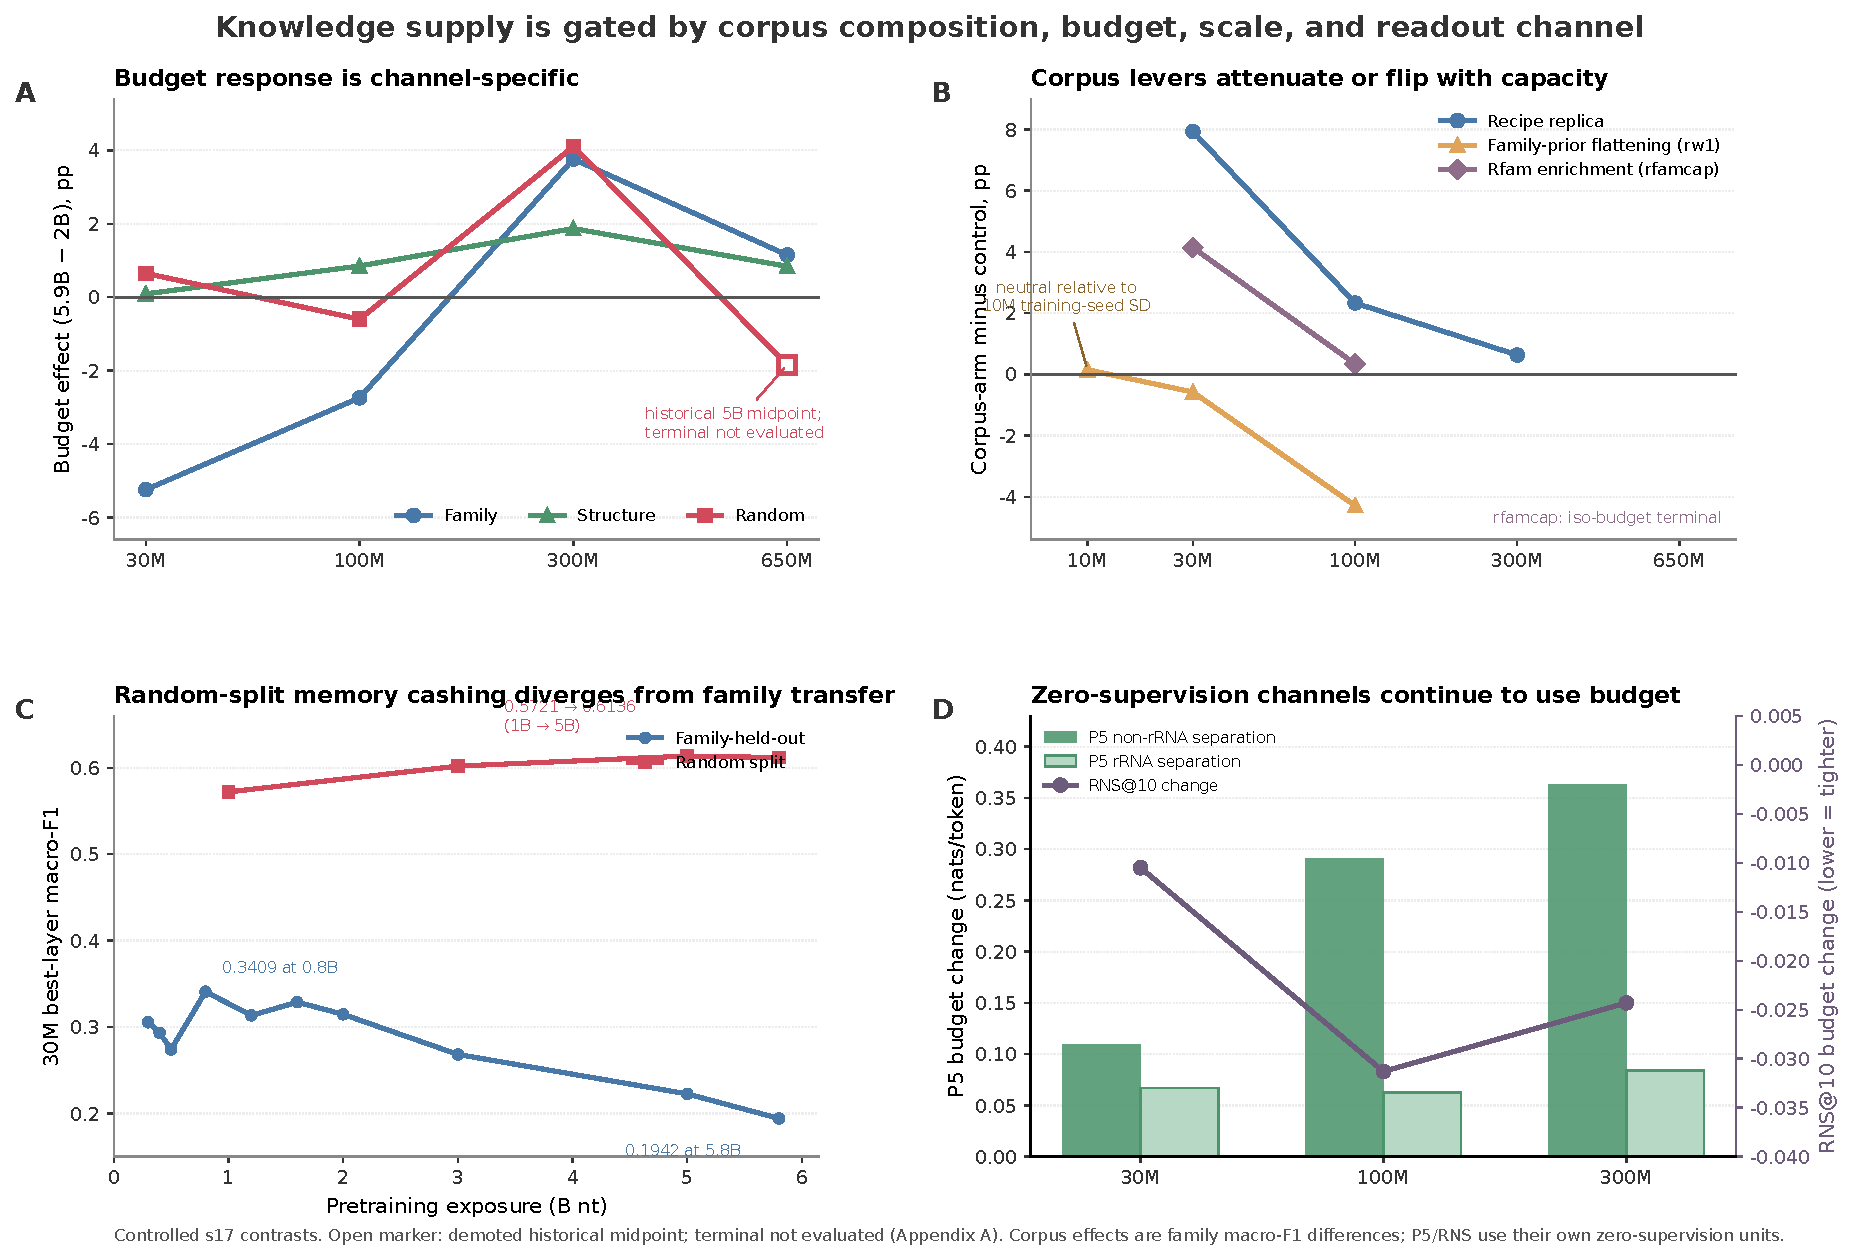
\includegraphics[width=\linewidth]{figs/fig5_q6_supply.pdf}
\caption{What determines knowledge supply? (A) Family, structure, and random-split responses to the 5.9B-versus-2B budget intervention; the open 650M random point is a demoted historical 5B midpoint, not a terminal result. (B) Controlled corpus-arm effects, including the monotone recipe-replica gradient, the capacity-dependent rw1 sign reversal, and terminal iso-budget rfamcap contrasts. (C) Divergent 30M random-split and family-held-out trajectories during continued pretraining. (D) Budget-induced RNS tightening and P5 shuffle-separation gains, showing that zero-supervision channels continue to respond after the family-classification plateau. Controlled contrasts use s17 runs; axes retain the native units of each channel rather than normalizing unlike metrics.}
\label{fig:5}
\end{figure}

Across these experiments, knowledge supply is not a scalar function of data volume: family, random-split, and structure responses are different projections of the same corpus-composition \(\times\) budget \(\times\) scale interaction onto distinct readout channels.

These channel-specific projections force the cross-cutting diagnostics in \S4.7, where representation organization and confidence must be assessed on their own axes rather than inferred from downstream F1. This section cannot establish an unconditional corpus-versus-parameter law, identify an optimal budget for every scale, or attribute the external +0.10 structure gap to corpus composition. The 650M random terminal point is unevaluated and the retest is unreviewed; both are stopped under the final split adjudication rather than presented as forthcoming, while the rfamcap structure checkpoint has been adjudicated.

\hypertarget{cross-cutting-diagnostics-representation-organization-and-confidence-do-not-identify-downstream-utility}{%
\subsection{Cross-cutting diagnostics: representation organization and confidence do not identify downstream utility}\label{cross-cutting-diagnostics-representation-organization-and-confidence-do-not-identify-downstream-utility}}

This cross-cutting section asks whether representation geometry or likelihood confidence can stand in for downstream usefulness, thereby testing the protein-derived diagnostics that motivate H7 and H8 rather than adding another rung to the Q1--Q6 chain. The decisive experiments are S14, which measures random-neighbor share (RNS) across scale, training time, models, families, and sequence bins, and S13b, which applies a pre-registered bell-curve decision rule to family-level masked negative log-likelihood (NLL) and structure F1. The joint phenomenon is a dissociation: RNS becomes tighter without tracking transfer across every axis, while the confidence--structure relation remains NOT-BELL because the sampled RNA models never reach the fitted high-NLL regime.

\hypertarget{rns-improves-with-scale-but-does-not-track-family-transfer}{%
\subsubsection{RNS improves with scale but does not track family transfer}\label{rns-improves-with-scale-but-does-not-track-family-transfer}}

RNS@10 measures the share of random sequences among a real sequence's nearest neighbors; lower values therefore indicate tighter organization of the real pool. Across the controlled endpoints, it decreases monotonically from 0.1721 at 1M to 0.1041, 0.0776, 0.0773, 0.0667, and 0.0620 at 10M, 30M, 100M, 300M, and 650M, respectively. The near-equality at 30M and 100M creates a local shoulder even though family macro-F1 rises sharply between those scales, and the subsequent RNS decreases show that this shoulder is not a global representation ceiling. Random-initialization controls remain much less organized (RNS@10 = 0.5442--0.5803), while ten random-pool regenerations give standard deviations of only 0.0037--0.0049 at the three tested scales; these are descriptive geometry checks, not training-seed uncertainty estimates.

The training-time axis further separates organization from utility. At 10M, RNS@10 reaches its maximum (worst organization) at 1.0B nt (0.1283), one checkpoint after the family-F1 maximum at 0.5B nt (0.2549), before declining to 0.1041 at 1.9B nt. In contrast, the 300M and 650M trajectories decline monotonically over the four sampled checkpoints, from 0.1201 to 0.0814 and from 0.1373 to 0.0662, respectively. This capacity-dependent difference is consistent with the supply-and-capacity account developed in Q4 and Q6, but the time courses are single-run descriptive measurements and do not identify a causal mechanism by themselves.

Cross-model behavior supports only a model-level association. Across eight models, Spearman's correlation between RNS@10 and random-split family F1 is \(-\)0.5952 (rounded to \(-\)0.60), with lower RNS accompanying higher F1; excluding the RNA-FM outlier weakens the estimate to \(-\)0.3929. Because four points come from the controlled family and four from external models with unauditable pretraining exposure, this is an observational anchor rather than a controlled cross-architecture result. Within the 30M model, the family-level correlation is only \(-\)0.1916 across eight families, too weak to treat geometric separation as a general ranking of downstream family performance.

The former sequence-level RNS-binning direction is withdrawn. The historical high-versus-low increases are retained only as superseded calculations in Appendix A because the pair labels used one-based indices incorrectly and the probe heads were not seeded. Consequently, neither a reversal relative to proteins nor the previously proposed axis-dependent length-confound mechanism is adjudicated. The retained RNS evidence is restricted to the scale, training-time, cross-model, and family axes above and the direct RNS--COV association below; none of these results establishes a per-sequence uncertainty proxy with a transferable sign.

\textbf{Direct RNS--COV association is weak to moderate.} In the 30M model, per-sequence Spearman \(\rho=-0.2966\) with bootstrap 95\% CI \([-0.4732,-0.1128]\) (\(n=108\)) indicates that lower RNS accompanies stronger COV \(-\) CTRL, but the strength does not support RNS as a strong structural-reliability proxy. The historical \texttt{s14\_rns\_cov.json} contains masked-marginal NLL rather than COV and is not evidence for this association; the new test uses actual mutation COV and remains within its own sequence protocol.

\hypertarget{the-pre-registered-confidence-bell-is-absent-within-the-sampled-nll-domain}{%
\subsubsection{The pre-registered confidence bell is absent within the sampled NLL domain}\label{the-pre-registered-confidence-bell-is-absent-within-the-sampled-nll-domain}}

S13b tests whether structure F1 first rises and then falls as masked NLL increases, the confidence-mediated pattern motivating the protein comparison \citep{hou_scaling}. The v1 fit contains 30 trained-model family points and places its quadratic vertex at NLL = 1.745, outside the observed range of approximately 1.34--1.38; it therefore returns the pre-registered NOT-BELL decision. Adding the 650M points in v2 gives 36 trained-model family points, widens the trained-point NLL range to 1.025--1.3872, and still places the vertex outside the data at 1.7201, again NOT-BELL under the same rule. The additional points broaden confidence coverage but are not independent training-seed replications, so they strengthen the domain-coverage check without upgrading the underlying descriptive evidence.

The negative result has a specific mechanistic interpretation: within this corpus and budget, the models do not sample the high-NLL, over-confident regime required for a descending right-hand limb, so the precondition for transferring Hou et al.'s protein account is unmet. It does not imply that RNA representations lack pairing knowledge, nor does it prove that no bell could appear under a different corpus, budget, task, or confidence measure; this boundary is consistent with the direct forward and paired-readout evidence in Q5. Likewise, family-level RNS is nearly unrelated to masked-marginal NLL (Spearman \(\rho=0.1429\), Pearson \(r=-0.0186\)), reinforcing that geometry, likelihood confidence, and downstream utility are distinct measurement axes.

\begin{figure}[htbp]
\centering
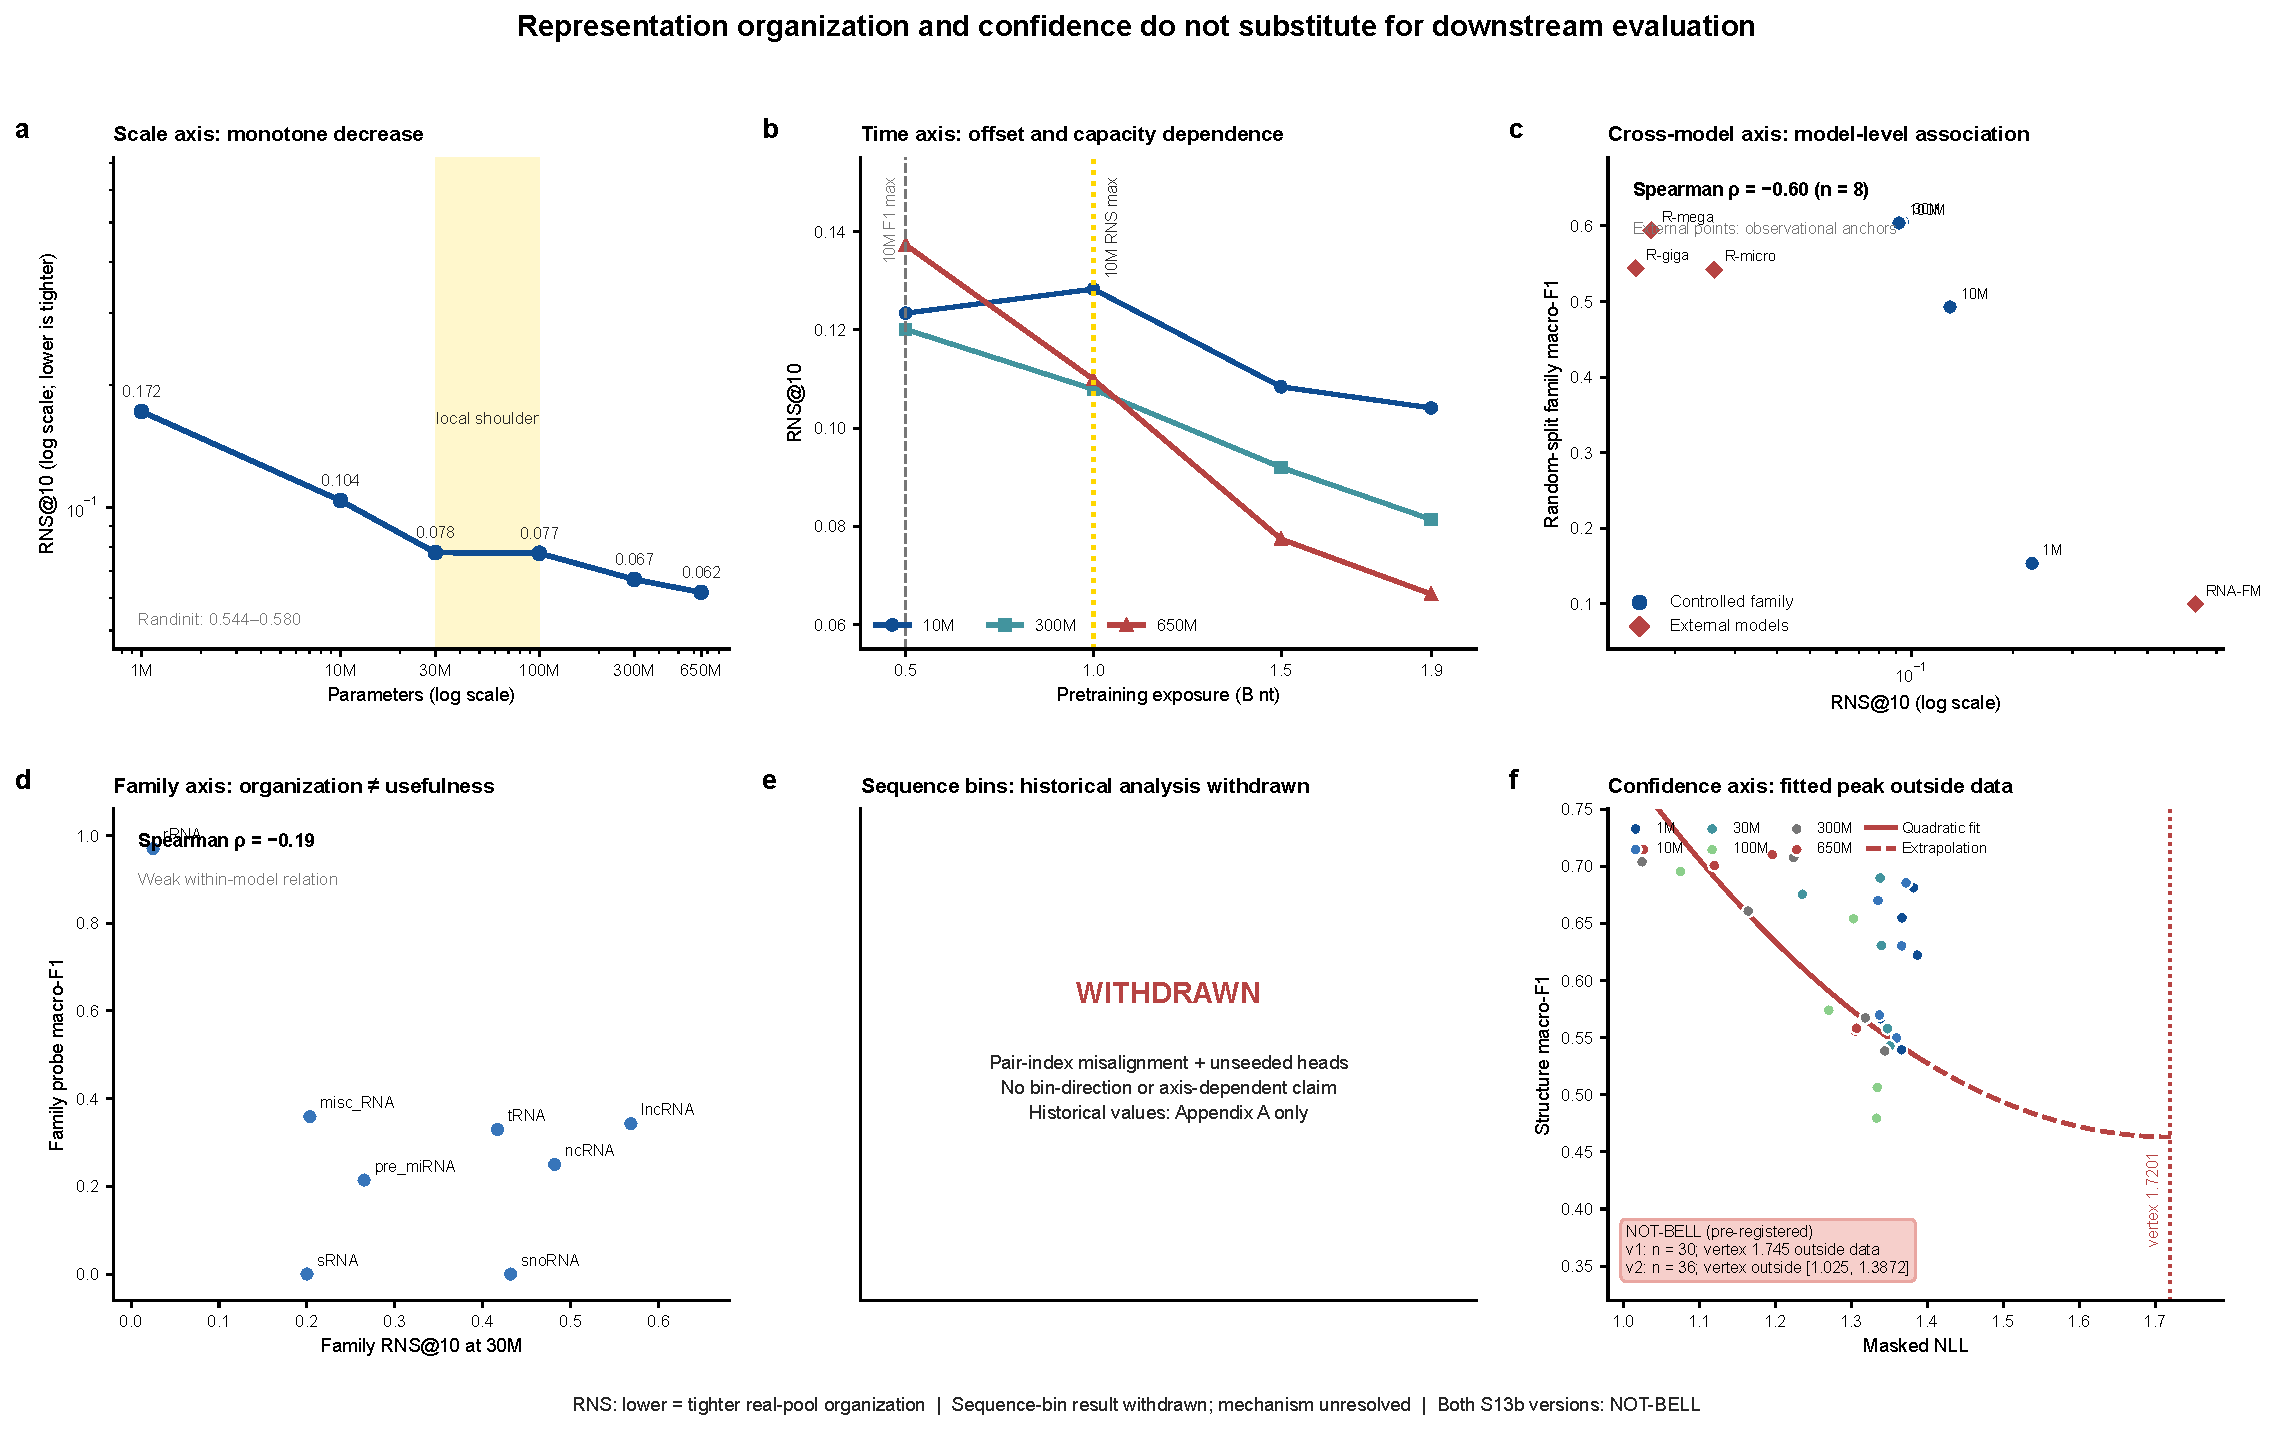
\includegraphics[width=\linewidth]{figs/fig6_crosscut.pdf}
\caption{Can representation geometry or likelihood confidence substitute for downstream evaluation? Panels show the RNS scale axis, training-time axis, cross-model and family associations, the withdrawn sequence-binning analysis, and the S13b confidence--structure fit. Lower RNS denotes tighter real-sequence organization; the 30M--100M shoulder is channel-specific. The binning panel retains no effect values or directional claim because pair-index misalignment and unseeded heads invalidate the historical analysis, leaving the axis-dependent mechanism unresolved. Both v1 and v2 retain the pre-registered NOT-BELL outcome because their fitted vertices lie outside the observed NLL ranges.}
\label{fig:6}
\end{figure}

These diagnostics lead directly to the integrated discussion: supply, representation organization, confidence, and readout must be treated as interacting but non-interchangeable components of transfer. They cannot establish a universal RNS--utility relationship, a sequence-level uncertainty estimator, a causal capacity mechanism, or the absence of confidence-mediated behavior outside the evaluated RNA domain.

\hypertarget{discussion}{%
\section{Discussion}\label{discussion}}

This discussion integrates Q1--Q6 and the cross-cutting diagnostics into one claim: RNA language-model transfer is real but gated knowledge supply, multiplied conceptually by protocol- and channel-dependent readout. The decisive evidence is the convergence of controlled initialization, split, corpus, budget, de-rRNA, mutation, and readout interventions, rather than any single scale curve or external-model comparison. The common phenomenon is that the same supply--readout interaction appears as a plateau, an attrition regime, a layer reversal, a budget-sign reversal, or a structural readout wall depending on which channel is measured.

The three apparent 30M plateaus provide the clearest projection of this interaction. At the original 2.0B-nt budget, the random-minus-family split dividend, RNS organization, and rRNA shuffle separation all flatten near 30M, but additional budget moves RNS and non-rRNA shuffle separation while family-transfer effects change sign across scale (\(-\)5.24, \(-\)2.74, +3.76, and +1.15 pp at 30M, 100M, 300M, and 650M). The completed random-split endpoints are comparatively insensitive to budget at the three smaller scales, whereas structural readout improves monotonically over those scales and remains positive at 650M. Thus, saturation of a family-classification or protocol-realized memory channel coexists with continued supply to other representation channels; it is not a global ceiling on what the models can learn.

The 10M attrition regime and the 650M shallow endpoint are two further projections of supply meeting capacity and corpus composition. The 10M endpoint is below the 1M endpoint only at the three-training-seed mean level, and its mid-training family-F1 maximum at 0.5B nt shows that prolonged exposure can erode a transiently readable family signal without a corresponding collapse in the structure task. At 650M, the best family readout shifts to relative depth 0.296 despite a higher endpoint score; removing rRNA from training and evaluation returns the best layer to L27 (relative depth 1.00) with de-rRNA F1 = 0.4585. This intervention supports the corpus-majority-occupancy component of the post-hoc capacity-reallocation account, but it does not validate the account's complete three-chain quantitative form, which has been falsified.

The structural results show why supply cannot be inferred from a single probe. Forward covariation reaches +0.0957 at 650M and remains near zero under random initialization, while partner-dependent readouts cluster near 0.64 despite a Partner-Oracle of 0.998 and a matched-prior pair-probe increment of +0.030. The same pretrained weights therefore contain pairing knowledge that a linear position classifier only partially exposes. The limiting readout operation is candidate-pair generation and matching, so a low linear-probe score is not a measurement of the total structural knowledge supplied by pretraining.

Corpus interventions complete the account by showing that supply itself is steerable but scale-dependent. The controlled recipe-replica contrast gains +7.93, +2.33, and +0.63 pp at 30M, 100M, and 300M, while the iso-budget rfamcap family contrast gains +4.14 and +0.34 pp at 30M and 100M. Conversely, flattening family frequencies changes family F1 by +0.15, \(-\)0.58, and \(-\)4.29 pp at 10M, 30M, and 100M, a capacity-gated sign reversal rather than a universal benefit of diversity. These controlled interventions justify prioritizing corpus recipe and budget placement within the evaluated family; external models remain observational anchors whose corpora, architectures, and exposures cannot be separated.

The cross-cutting RNS and NOT-BELL results prevent this integration from becoming a claim that one geometric or likelihood scalar can replace downstream evaluation. Representation organization can tighten while family transfer follows a different trajectory, and the confidence--structure bell is absent because its required regime lies outside the sampled NLL range. The former sequence-binned RNS direction is withdrawn because pair indices were misaligned and probe heads were not seeded; the proposed axis-dependent mechanism is therefore unresolved. The integrated claim is consequently about distinct supply and readout channels supported by the retained RNS axes and direct RNS--COV association, not about a single latent ``representation quality'' variable.

These conclusions make the remaining uncertainties---composition non-separability, external-corpus exposure, incomplete corpus arms, uneven seed coverage, and unresolved checkpoint provenance---the immediate next objects of evaluation rather than minor caveats. The study cannot establish a universal scaling law, a complete capacity-allocation mechanism, architecture-independent corpus effects, or the performance obtainable with a dedicated pairing solver.

For model development in this setting, the priorities are (1) choose the corpus recipe, (2) place the training budget at the appropriate point for the target scale, (3) select the evaluation protocol and a readout head matched to the required operation, and only then (4) choose parameter count, with the limitations above defining the next confirmatory tests. The companion rna-ft-eval study separately evaluates fine-tuning, freezing, and LoRA recipes; this paper supplies the controlled pretraining and readout evidence, and neither study's mechanism claims are imported into the other or extended beyond its own evidence.

\hypertarget{limitations}{%
\section{Limitations}\label{limitations}}

This section asks which conclusions remain under-identified after the controlled interventions and which reporting gaps constrain their interpretation. The decisive audit crosses composition baselines, external-corpus exposure, unfinished arms, training-seed coverage, epoch coverage, rRNA stratification, readout protocols, and checkpoint-level provenance. The resulting picture is that every main claim has an explicit boundary control, but none of those controls licenses extrapolation beyond the measured arms, protocols, and evidence grades.

\begin{longtable}[]{@{}
  >{\raggedright\arraybackslash}p{(\columnwidth - 4\tabcolsep) * \real{0.33}}
  >{\raggedright\arraybackslash}p{(\columnwidth - 4\tabcolsep) * \real{0.33}}
  >{\raggedright\arraybackslash}p{(\columnwidth - 4\tabcolsep) * \real{0.33}}@{}}
\toprule
Limitation & Consequence for interpretation & Boundary control already applied \\
\midrule
\endhead
\textbf{B3: learned weight structure and composition reading are not separable.} Randinit and moment-matched controls establish that the advantage requires learned weights, but neither control reads sequence composition; classical baselines can therefore capture overlapping signal. & A positive trained-minus-control effect is not automatically a beyond-composition effect, and the family-split margin depends on baseline and protocol. & S9 crosses split and protocol with k-mer logistic regression, LightGBM, a supervised one-hot CNN, and random embeddings, while S4/S5 provide the intervention arm. The primary mean-pool contrast explicitly uses LightGBM s17 only; balanced s17 sensitivity is reported separately rather than replacing it with the former k-mer comparison. \\
\textbf{External pretraining corpora are a bidirectional black box.} Published models may contain homologues of the evaluation families, while their sequence manifests cannot be audited against the S0 partitions. & External scores can be affected in either direction by unknown exposure and are jointly confounded by architecture, corpus, and training budget; they cannot support controlled corpus attribution. & Cluster and exact-sequence isolation is asserted only for the self-trained family. The new external COV gradient and its randinit controls are labeled observational anchors; controlled corpus claims continue to use same-architecture recipe-replica and rfamcap arms instead. \\
\textbf{The rfamcap structure effect does not explain the cross-model structure gap.} The adjudicated terminal rfamcap-minus-main differences are +1.77 pp at 30M and +0.14 pp at 100M under paired-F1, whereas the external gap under discussion is approximately +0.10 F1. & Corpus enrichment alone is insufficient to account for that cross-model difference; architecture, corpus source, exposure, and readout remain confounded. & The rfamcap arm retains the architecture and provides same-seed terminal contrasts with randinit floors in place. Both family and structure effects decay with capacity, but the single-seed TS0 best-layer structure results remain descriptive and are not used to attribute the external gap. \\
\textbf{The historical rfamcap structure result is not reproducible.} Neither the 1.8B nor the 1.9B candidate checkpoint reproduced any of the 23 historical layers (0/23 exact-layer matches for each). & The historical \texttt{0.5924@L20} and its +0.34 pp contrast are withdrawn; only the new terminal paired-F1 contrasts are current. & The checkpoint adjudication directly evaluated both candidates and added the missing 30M structure arm. This resolves the former checkpoint-label gap without claiming that the unknown historical source has been identified. \\
\textbf{MARS and RNAcentral corpus arms are unfinished.} MARS has no completed terminal probes, and RNAcentral has no retrievable checkpoints in the authoritative backup; several MARS arms retain only low-budget midpoints. & The evidence does not support a three-corpus spectrum or terminal comparisons for these arms. & A run-level registry records zero probe rows, available checkpoints, and empty directories. No missing arm is treated as a negative result; the corpus claim remains restricted to the main recipe, the recipe replica, and the rfamcap orthogonal point. \\
\textbf{Training-seed coverage is uneven at 300M and 650M.} Both tiers contain only training seed s17. & Their endpoint differences, saturation, layer locations, and budget responses have no training-seed uncertainty estimate. & Single-seed entries are shown without fabricated error bars and are separated from the three-training-seed 1M--100M summaries. The unreviewed probe-seed retest is excluded from current evidence and is not independent pretraining replication. \\
\textbf{The 10M attrition is a mean-level phenomenon.} The 10M mean is below the 1M mean, but the paired change is negative in only two of three training seeds. & A universal per-seed decline or a precise seed-invariant magnitude is not supported. & The three paired training seeds are retained in the main table, the time axis locates a 0.5B-nt family-F1 maximum, the c1Mcs arm tests repeated exposure, and structure probing provides a task-specificity control. \\
\textbf{Unique-corpus size and epoch coverage covary.} Smaller-corpus arms can receive more epochs at the same nucleotide budget, so corpus quantity, repetition, and training duration are not interchangeable variables. & A corpus-size ranking cannot be interpreted as a pure unique-data effect across unmatched coverage. & Saturation comparisons are restricted to matched exposure/coverage, the c1Mcs repeated-exposure arm is used to test the duration account, and epoch counts accompany corpus-axis interpretations rather than being hidden by iso-token labels. \\
\textbf{The corpus is rRNA-biased.} A dominant rRNA channel can shape both absolute family scores and the layer at which non-rRNA family signal is easiest to read. & Full-corpus scores need not represent non-rRNA transfer, and deep-layer relocation cannot be interpreted without corpus stratification. & De-rRNA stratified reanalysis preserves the headline scale, mean-level attrition, and layer-shape directions, although absolute scores decrease. The P1 de-rRNA intervention removes the 650M shallow endpoint, directly testing the corpus-channel component while leaving the broader post-hoc quantitative account unconfirmed. \\
\textbf{Mean-pool results support only within-protocol, relative conclusions.} Pooling and head choice are readout interventions, not neutral implementations. & Absolute scores and baseline margins cannot be transferred between mean-pool and balanced protocols. & Both protocols are evaluated explicitly; for example, balanced s17 at 100M gives LM 0.1696 versus LightGBM 0.1760, whereas the adjudicated primary baseline table uses the separate mean-pool caliber. No cross-protocol difference is interpreted as a training effect. \\
\textbf{The 650M extended-budget retest is unreviewed and uses a different probe protocol.} Its summary values lack designated raw JSONL ledger rows, and the retest changes probe seeds, sample count, and layer-search window. & The retest supplies no current 650M-over-300M claim, training-seed replication, readout-stability conclusion, or same-protocol budget effect. & The factorial headline retains only the original terminal-protocol +1.15 pp single-seed E1 effect. Retest summaries are demoted to a handover-record citation in Appendix A rather than described as pending consolidation. \\
\textbf{The original split file is unrecoverable, and reconstruction is not equivalent.} The original member-to-representative mapping, clustering parquet, executable binary, and complete run log are missing. Although sequence content is recovered, the reconstructed cluster topology differs and places former training sequences in family-validation and family-test, violating pretraining-held-out isolation. & P2.5 retest consolidation and P2.7 random-terminal evaluation are stopped and demoted; P2.4 length-controlled RNS binning is not performed and its historical direction is withdrawn. P3.1 multi-seed training is not triggered because training on the reconstructed split would be leaky and incomparable, while a new data version would require retraining every comparison arm. & The final split adjudication preserves the reconstruction assets for future acceptance only if the original member mapping is recovered. No surrogate split is substituted, no leakage-affected probe is treated as valid, and the stopped analyses are not reported as negative results. \\
\bottomrule
\end{longtable}

These limitations lead directly to the provenance appendix, which preserves superseded values and protocol differences without allowing them to compete with the adjudicated main results. They prevent claims of composition-independent transfer, controlled external-corpus attribution, training-seed-robust large-scale effects, universal per-seed attrition, finalized retest provenance, a 650M random-terminal response, or an adjudicated RNS-binning mechanism. The rfamcap structure checkpoint is adjudicated, and external COV and RNS\(\times\)COV are included with their observational limits; the unrecoverable split is an explicit evidence gap rather than unfinished work presented as forthcoming.

\appendix
\hypertarget{appendix-a.-provenance-of-superseded-values-and-reporting-calibers}{%
\section{Provenance of superseded values and reporting calibers}\label{appendix-a.-provenance-of-superseded-values-and-reporting-calibers}}

This appendix records which historical numbers were replaced or demoted during P0 adjudication and why they must not be mixed with the current results. The decisive sources are the frozen contradiction audit at old-DRAFT lines L598--L622, the standard-deviation and 650M retest recalculation, and the rfamcap iso-budget correction. The central provenance observation is that most discrepancies arise from changed comparators, checkpoints, protocols, or degrees of freedom rather than from new training runs.

\hypertarget{a.1-structural-readout-audit-at-old-draft-l598l622}{%
\subsection{Structural-readout audit at old DRAFT L598--L622}\label{a.1-structural-readout-audit-at-old-draft-l598l622}}

The old composition-floor vector \texttt{1M\ \(-\)0.047\ /\allowbreak\ \ 10M\ \(-\)0.010\ /\allowbreak\ \ 30M\ \(-\)0.000\ /\allowbreak\ \ 100M\ +0.013\ /\allowbreak\ \ 650M\ +0.021} (L606--L608) is \textbf{superseded} and must not be used as a current scale result. The 1M row used a weak training subset (35k tokens versus 1.0M for the other scales), and the earlier comparison mixed paired-class F1 with a macro-F1 floor; a separate first multi-dataset run was excluded because sequence and pair labels were shuffled with different seeds (old DRAFT L345--L352; P0.5/C1--C2). The corrected own-best trained-minus-randinit values are \texttt{1M\ +0.007\ /\allowbreak\ \ 10M\ \(-\)0.001\ /\allowbreak\ \ 30M\ \(-\)0.003\ /\allowbreak\ \ 100M\ +0.004}, a comparator-specific linear-readout result rather than a cross-channel estimate of pairing knowledge.

The corrected 1M \texttt{+0.007} above must not be confused with the old \textbf{family-classification baseline} \texttt{+0.007} at 100M. The latter compared balanced-probe LM s17 (approximately 0.170) with k-mer logistic regression (0.163), whereas the strongest observed classical comparator was LightGBM s17 at 0.1760; under the same balanced s17 protocol, LM = 0.1696 and the contrast is \(-\)0.0064 (P0.3). That old family-baseline \texttt{+0.007} is therefore \textbf{demoted to a non-primary historical comparator}, while the structurally distinct own-best trained-minus-randinit \texttt{+0.007} remains valid only with its comparator named. The current primary mean-pool observed-baseline contrast at 100M is +0.1634 using the three-training-seed LM mean against LightGBM s17, not a three-seed-versus-three-seed comparison.

The old inference that paired knowledge was broadly absent is \textbf{withdrawn}, not preserved as an alternative current conclusion. Later forward covariation, Partner-Oracle, and matched-prior pair-probe evidence establish pretraining-derived pairing signal while retaining the narrower finding that linear readout exposes only a small net increment at the tested scales (P0.5/C1). The numerical history is retained here for traceability without reproducing the withdrawn wording.

\hypertarget{a.2-rfamcap-checkpoint-and-budget-caliber}{%
\subsection{Rfamcap checkpoint and budget caliber}\label{a.2-rfamcap-checkpoint-and-budget-caliber}}

The rfamcap 100M midpoint value \texttt{0.3448@L18} at 0.2B nt and its \texttt{+1.85\ pp} contrast against main-line 100M \texttt{0.3263@L21} are \textbf{demoted to trajectory observations}. The comparator was a 1.9B terminal checkpoint, so the difference mixed corpus composition with budget; the main arms also lack matched 0.2B checkpoints, preventing a clean midpoint comparison (P0/B1). The adjudicated iso-budget terminal values are rfamcap \texttt{0.3297@L13} versus main \texttt{0.3263@L21}, giving \texttt{+0.34\ pp} at 100M; at 30M, the terminal rfamcap value is \texttt{0.2880@L8}, giving \texttt{+4.14\ pp} against \texttt{0.2466@L8}.

The historical rfamcap 100M structure value \texttt{0.5924@L20}, and hence its \texttt{+0.34\ pp} difference from main \texttt{0.5890@L22}, is \textbf{withdrawn}, not merely checkpoint-unresolved. Neither the 1.8B nor the 1.9B candidate checkpoint reproduced any historical layer (0/23 exact-layer matches for each), and the historical source checkpoint remains unknown. The current 1.9B terminal contrasts instead use paired-F1: at 30M, rfamcap \texttt{0.5933@L11} versus main \texttt{0.5756@L3} gives \texttt{+1.77\ pp}; at 100M, rfamcap \texttt{0.5904@L22} versus main \texttt{0.5890@L22} gives \texttt{+0.14\ pp}. These new values supersede the historical structure effect and are reported separately from true macro-F1.

\hypertarget{a.3-standard-deviation-conventions}{%
\subsection{Standard-deviation conventions}\label{a.3-standard-deviation-conventions}}

The population-standard-deviation versions \texttt{0.0107\ /\allowbreak\ \ 0.0141\ /\allowbreak\ \ 0.0132\ /\allowbreak\ \ 0.0120} at 1M/10M/30M/100M (ddof=0) are \textbf{replaced in main-text summaries} by the sample-standard-deviation values \texttt{0.0131\ /\allowbreak\ \ 0.0173\ /\allowbreak\ \ 0.0162\ /\allowbreak\ \ 0.0147} (ddof=1). Both versions use the same 12 training-seed best-layer F1 values and final checkpoints; their ratio is exactly \(\sqrt{3/2}\), so the discrepancy is purely the denominator convention (P0.2a). The ddof=0 values remain reproducible alternative summaries, not independent uncertainty measurements and not standard errors.

\hypertarget{a.4-the-650m-extended-budget-protocols}{%
\subsection{The 650M extended-budget protocols}\label{a.4-the-650m-extended-budget-protocols}}

Under the original terminal protocol (20,000/4,000 probe sequences, full-layer scans, probe seed 17), 650M at 5.9B scores \texttt{0.3747@L25}, below 300M at \texttt{0.3821@L22} by \texttt{\(-\)0.74\ pp}. This original result is \textbf{valid but protocol-specific}, not superseded: it remains the factorial input and yields the same-protocol 650M budget effect \texttt{0.3747\ \(-\)\ 0.3632\ =\ +1.15\ pp} (P0.2b). Duplicate ledger rows were deduplicated and are not additional seeds.

The deep-window retest instead uses 8,000/4,000 sequences and probe seeds 29/43/61 on the same s17 trained weights, giving 650M \texttt{0.4491\ \(\pm\)\ 0.0147} versus 300M \texttt{0.3826\ \(\pm\)\ 0.0159}, a \texttt{+6.65\ pp} mean paired difference with three of three probe-seed pairs positive. These values are \textbf{demoted to an unreviewed handover-record citation} and are not current evidence for readout stability, a 650M-over-300M advantage, training-seed replication, or sequence-bootstrap uncertainty. All 30 seed--layer values lack corresponding rows in the designated raw JSONL ledger; P2.5 consolidation is stopped because the original split cannot be recovered and the leaky reconstruction cannot support an equivalent retest.

The descriptive difference \texttt{0.4491\ \(-\)\ 0.3632\ =\ +8.59\ pp} is \textbf{invalid as a budget-effect headline} because it crosses probe protocols, sample counts, layer windows, and probe-seed rules. Only \texttt{+1.15\ pp} enters the original-terminal factorial table; a retest-based budget effect would require applying the same retest protocol to the 2.0B weights. The earlier \texttt{+6.5\ pp} rendering of the 650M-minus-300M retest difference is also replaced by the correctly rounded \texttt{+6.65\ pp} (or \texttt{+6.6\ pp} to one decimal).

The 650M random-split value \texttt{\(-\)1.85\ pp} is a \textbf{demoted historical 5B midpoint observation} (\texttt{0.6067} at 5B minus the 2B terminal value \texttt{0.6252}), not a terminal budget effect. P2.7 is stopped because the original split is unrecoverable and the reconstruction leaks former training sequences into evaluation partitions. The random-channel budget-insensitivity claim is therefore restricted to the three completed terminal comparisons; the open point in Figure 5 is a visual provenance marker for this appendix observation, not a fourth terminal result.

\hypertarget{a.5-withdrawn-rns-sequence-binning-analysis}{%
\subsection{Withdrawn RNS sequence-binning analysis}\label{a.5-withdrawn-rns-sequence-binning-analysis}}

The historical 100M low/middle/high RNS-bin paired-position F1 values \texttt{0.4005/0.5011/0.4727} and long-range F1 values \texttt{0.5735/0.7430/0.7414}, together with the high-versus-low increases \texttt{+18.0\%} and \texttt{+29.3\%}, are \textbf{withdrawn to historical reference only}. The pair labels used one-based indices incorrectly and the probe heads were not seeded. These values must not support a sequence-binning direction, a reversal relative to proteins, or an axis-dependent mechanism. The historical length--RNS Spearman value \texttt{+0.1915} is likewise insufficient to adjudicate the proposed length-confound account. P2.4 length-controlled reanalysis is not performed under the final split adjudication. The RNS scale, training-time, cross-model, and family axes and the separate direct RNS--COV analysis are unaffected.

\hypertarget{a.6-final-split-adjudication}{%
\subsection{Final split adjudication}\label{a.6-final-split-adjudication}}

The original split cannot be exactly restored because its member-to-representative mapping, original clustering parquet, executable binary, and complete run log are unavailable. Reconstruction recovers sequence content but changes cluster topology and introduces observable train-to-family-validation/test leakage, so it cannot be used to probe old checkpoints as though pretraining-held-out isolation still held. Accordingly, P2.5 and P2.7 are stopped and demoted, P2.4 is not performed and its binning claim is withdrawn, and P3.1 multi-seed supplementation is not triggered. A future new data version would require fresh preregistration and retraining of all comparison arms; these stopped analyses are neither completed nor negative results.

\hypertarget{a.7-status-key}{%
\subsection{Status key}\label{a.7-status-key}}

\textbf{Superseded} values are replaced because of a corrected metric, training subset, or statistical convention; \textbf{withdrawn} values fail reproduction or lose inferential validity and must not be used as current evidence; \textbf{demoted} values remain descriptive observations but lose causal or primary-table status because their comparators or checkpoints differ; \textbf{valid but protocol-specific} values remain current only inside their stated protocol; and \textbf{unreviewed handover-record} values are preserved for traceability without raw-ledger or split-file verification. These labels implement P0.5/C1--C2, P0/A1--A2/B1, and the final split adjudication without deleting negative or protocol-sensitive results.

This appendix closes the provenance trail for the limitations and prevents historical values from re-entering the Results as current evidence. It cannot repair the missing retest ledger rows, restore the original split, reproduce the withdrawn historical rfamcap structure value or identify its unknown source, create matched midpoints, validate the historical RNS-binning direction, or convert probe-seed repetition into independent training-seed replication.


\bibliographystyle{plainnat}
\bibliography{refs}

\end{document}
